\documentclass[12pt]{amsart}

\usepackage{enumerate,amsmath,amssymb,amsthm,mathtools,comment}
\usepackage{simpler-wick}

\usepackage{arydshln}
\usepackage{dashrule}
\usepackage{slashed}
\usepackage{mathrsfs}
%for Griffiths curly r
\usepackage{calligra}
\DeclareMathAlphabet{\mathcalligra}{T1}{calligra}{m}{n}
\DeclareFontShape{T1}{calligra}{m}{n}{<->s*[2.2]callig15}{}
\newcommand{\scripty}[1]{\ensuremath{\mathcalligra{#1}}}



\newcommand{\capk}{\frac{1}{4 \pi \epsilon_0}}

\begin{document}
\title{}
%\author{Alec Hewitt}
\maketitle

\setlength{\parindent}{0mm}



\begin{enumerate}
\setcounter{enumi}{892}

\item \underline{$\frac{\partial \mathcal{L}}{\partial \phi} - \partial_{\mu} ( \frac{\partial \mathcal{L}}{\partial ( \partial_{\mu} \phi)})=0$}\\
$L = \int \mathcal{L} d^3 x,\,\, \mathcal{L}$ is called the Lagrangian density, where $\mathcal{L} = \mathcal{L} (\phi, \partial_{\mu} \phi)\\$
$S = \int L dt = \int \mathcal{L} d^4 x\\
\delta S = \int ( \frac{\partial \mathcal{L}}{\partial \phi} \delta \phi + \frac{\partial \mathcal{L}}{\partial ( \partial_{\mu} \phi)} \delta ( \partial_{\mu} \phi)) d^4 \\
\delta( \partial_{\mu} \phi) = \partial_{\mu} \delta \phi\\
= \int [ \frac{\partial \mathcal{L}}{\partial \phi} \delta \phi + \frac{\partial \mathcal{L}}{\partial ( \partial_{\mu} \phi)} \partial_{\mu} ( \delta \phi) ] d^4 x\\
\partial_{\mu} ( \frac{\partial \mathcal{L}}{\partial ( \partial_{\mu} \phi)} \delta \phi)\\
= \partial_{\mu} ( \frac{\partial \mathcal{L}}{\partial ( \partial_{\mu} \phi)}) \delta \phi + \frac{\partial \mathcal{L}}{\partial ( \partial_{\mu} \phi)} \partial_{\mu} ( \delta \phi)\\
= \int [ \frac{\partial \mathcal{L}}{\partial \phi} \delta \phi + \partial_{\mu} ( \frac{\partial \mathcal{L}}{\partial ( \partial_{\mu} \phi)} \delta \phi )- \partial_{\mu} ( \frac{\partial \mathcal{L}}{\partial ( \partial_{\mu} \phi)}) \delta \phi] d^4 x\\
= \int [ \frac{\partial \mathcal{L}}{\partial \phi} - \partial_{\mu}( \frac{\partial \mathcal{L}}{\partial ( \partial_{\mu} \phi)}) ] \delta \phi d^4 x\\
\implies \frac{\partial \mathcal{L}}{\partial \phi} - \partial_{\mu}( \frac{\partial \mathcal{L}}{\partial ( \partial_{\mu} \phi)}) =0\\$


\hdashrule[0.5ex][c]{\linewidth}{0.5pt}{1.5mm}


\item \underline{$\hat{H} = \sum_{k=1}^N \hbar \omega_k ( a_k^{\dagger} a_k + \frac{1}{2})$}\\
\underline{recall:} $\hat{H} = \sum_j \frac{\hat{p}_j^2}{2m} + \frac{1}{2} k ( \hat{x}_{j+1} - \hat{x}_j)^2$ (Hamiltonian for 1-D lattice connected by springs)\\
replace w/ Fourier transforms also Note that $\tilde{x} \rightarrow \hat{x}$ (Notation)\\
$\hat{H} = \sum_k [ \frac{1}{2m} \hat{p}_k \hat{p}_{-k} + \frac{1}{2} m \omega_k^2 \hat{x}_k \hat{x}_{-k} ]$\\
Notice similarity from QM $H = \frac{p^2}{2m} + \frac{1}{2} m \omega^2 x^2\\
\implies \begin{cases} \hat{a}_k = \sqrt{ \frac{m \omega_k}{2 \hbar}} ( \hat{x}_k + \frac{i}{m \omega_k} \hat{p}_k)\\
\hat{a}_k^{\dagger} = \sqrt{ \frac{m \omega_k}{2 \hbar}} ( \hat{x}_k - \frac{i}{m \omega_k} \hat{p}_k) \end{cases}$\\
invert and insert (check this)\\
$\therefore \hat{H} = \sum_{k=1}^N \hbar \omega_k ( a_k^{\dagger} a_k + \frac{1}{2})\\$


\hdashrule[0.5ex][c]{\linewidth}{0.5pt}{1.5mm}


$\implies \hat{H} = \int d^3 p E_p \hat{a}_p^{\dagger} \hat{a}_p\\$


\hdashrule[0.5ex][c]{\linewidth}{0.5pt}{1.5mm}


\item \underline{$L = \int d^3 x [ \frac{1}{2} \rho ( \frac{\partial \phi}{\partial t})^2 - \frac{1}{2} \mathcal{T} ( \nabla \phi)^2]$}\\
\underline{recall:} $L = \sum_j \frac{p_j^2}{2m} - \frac{1}{2} k ( q_{j+1} - q_j)^2$ (easy to obtain from previous Hamiltonian)\\
$\sum_j \rightarrow \frac{1}{\ell} \int d x,\,\, \ell \sim$ dist between lattice points\\
$\sum_j \frac{p_j^2}{2m} = \sum_j \frac{1}{2} m ( \frac{\partial q_j}{\partial t})^2 \rightarrow \frac{1}{\ell} \int dx \frac{1}{2} m ( \frac{\partial \phi(x,t)}{\partial t})^2\\
\sum \frac{1}{2} k ( q_{j+1} - q_j)^2 \rightarrow \frac{1}{2} k \int d x ( \frac{q_{j+1} - q_j}{\ell})^2 = \frac{1}{2} \int d x k ( \frac{\partial \phi}{\partial x})^2 \ell\\
\implies L \rightarrow \int d^3 x [ \frac{1}{2} \rho ( \frac{\partial \phi}{\partial t})^2 - \frac{1}{2} \mathcal{T} ( \nabla \phi)^2]$


\hdashrule[0.5ex][c]{\linewidth}{0.5pt}{1.5mm}


\underline{recall:} $\mathcal{L} = \frac{1}{2} \rho ( \frac{\partial \phi}{\partial t})^2 - \frac{1}{2} T ( \nabla \phi)^2\\
T$ is like the bulk modulus $B$\\
$\implies \mathcal{L} = \rho[ \frac{1}{2} ( \frac{\partial \phi}{\partial t})^2 - \frac{1}{2} v^2 ( \nabla \phi)^2]$\\
if $\delta \mathcal{L} =0 \implies \rho$ doesn't matter\\
$\implies \mathcal{L} = \frac{1}{2}( \frac{\partial \phi}{\partial t})^2 - \frac{1}{2} ( \nabla \phi)^2$\\
$\implies \mathcal{L} = \frac{1}{2} \partial^{\mu} \phi \partial_{\mu} \phi$\\
this is the wave equation, or in other words it is a Klein gordon equation for a massless scalar field that travels at $c=1$ (the speed of light)
more generally,\\
\underline{recall:} $\mathcal{L} = \frac{1}{2} ( \partial_{\mu} \phi)^2 - \frac{1}{2} m^2 \phi^2$ (Klein-Gordon $\mathcal{L}$ for a $\underline{real}$ scalar field)\\


\hdashrule[0.5ex][c]{\linewidth}{0.5pt}{1.5mm}


\item  \underline{ $\tilde{\phi}( \vec{p}) = \frac{1}{\sqrt{2 E_{\vec{p}}}}( a_{\vec{p}} + a_{- \vec{p}}^{\dagger})$}\\
\underline{recall:} $a = \frac{1}{2} ( \sqrt{2 \omega} q + i \sqrt{ \frac{2}{\omega}} \pi)\\
q \sim$ position operator,$\,\, \pi \sim$ momentum operator\\
promote them to fields\\
(why promote them to fourier transforms $\tilde{\phi} of \phi?)\\
\implies a_{\vec{p}} = \frac{1}{2} ( \sqrt{ 2 \omega_{\vec{p}}} \tilde{\phi}(\vec{p}) + i \sqrt{ \frac{2}{\omega_{\vec{p}}} }\tilde{\pi}(\vec{p}))\\$
\underline{Note:} $\tilde{\phi}^{\dagger}(\vec{p}) = \tilde{\phi}(- \vec{p}) and \tilde{p}^{\dagger}( \vec{p}) = \tilde{\pi}( - \vec{p})\\$
(not sure why...)\\
$\implies 
\begin{cases}
a_{\vec{p}} = \frac{1}{2} ( \sqrt{2 \omega_{\vec{p}}} \tilde{\phi}( \vec{p})+ i \sqrt{ \frac{2}{\omega_{\vec{p}}}} \tilde{\pi} ( \vec{p}))\\
a_{- \vec{p}}^{\dagger} = \frac{1}{2} ( \sqrt{2 \omega_{\vec{p}}} \tilde{\phi}( \vec{p}) - i \sqrt{ \frac{2}{ \omega_{\vec{p}}}} \tilde{\pi}( \vec{p}))\\
\end{cases}\\
 $
\underline{Note:} I used $\omega_{- \vec{p}} = \omega_{\vec{p}}$\\
add \\
$\implies a_{\vec{p}} + a_{- \vec{p}}^{\dagger} = \sqrt{2 \omega_{\vec{p}} }\tilde{\phi}( \vec{p})\\
\therefore \tilde{\phi}(\vec{p}) = \frac{1}{\sqrt{2 E_{\vec{p}}}} ( a_{\vec{p}} + a_{- \vec{p}}^{\dagger})\\$


\hdashrule[0.5ex][c]{\linewidth}{0.5pt}{1.5mm}


\item \underline{$\phi(\vec{x}) = \int \frac{d^3 p}{(2 \pi)^3} \frac{1}{\sqrt{2 E_{\vec{p}}}} ( a_{\vec{p}}^{\dagger} e^{-i \vec{p} \cdot \vec{x}} + a_{\vec{p}} e^{i \vec{p} \cdot \vec{x}})$}\\
\underline{recall:} $\tilde{\phi}( \vec{p}) = \frac{1}{\sqrt{2 E_{\vec{p}}}} ( a_{\vec{p}} + a_{- \vec{p}}^{\dagger})$\\
now Fourier transform\\
$\phi(\vec{x}) = \int \frac{d^3 p}{(2 \pi)^3} e^{i \vec{p} \cdot \vec{x}} \tilde{\phi}( \vec{p})\\
= \int \frac{d^3 p}{(2 \pi)^3} e^{i \vec{p} \cdot \vec{x}} \frac{1}{\sqrt{2 E_{\vec{p}}}} ( \hat{a}_{\vec{p}} + \hat{a}_{- \vec{p}}^{\dagger})\\
= \int \frac{d^3 p}{(2 \pi)^3} \frac{1}{\sqrt{ 2 E_{\vec{p}}}} e^{i \vec{p} \cdot \vec{x}} \hat{a}_{\vec{p}} + \int \frac{d^3 p}{(2 \pi)^3} \frac{1}{\sqrt{2 E)_{\vec{p}}}} a_{- \vec{p}}^{\dagger} e^{i \vec{p} \cdot \vec{x}}\\
\int \frac{d^3 p}{(2 \pi)^3} \frac{1}{\sqrt{2 E_{\vec{p}}}} a_{-\vec{p}}^{\dagger} e^{i \vec{p} \cdot \vec{x}}\\
= \int_{- \infty}^{\infty} \int_{- \infty}^{\infty} \int_{- \infty}^{\infty} \frac{d^3 p}{(2 \pi)^3} \frac{1}{\sqrt{2 E_{\vec{p}}}} a_{- \vec{p}}^{\dagger} e^{i \vec{p} \cdot \vec{x}}\\
\vec{p}' = - \vec{p}\\
= \int_{\infty}^{- \infty} \int_{\infty}^{- \infty} \int_{\infty}^{- \infty} \frac{- d^3 p}{(2 \pi)^3} \frac{1}{\sqrt{2 E_{- \vec{p}}}} a_{\vec{p}}^{\dagger} e^{- i \vec{p} \cdot \vec{x}}\\
= \int \frac{d^3 p}{(2 \pi)^3} \frac{1}{\sqrt{2 E_{\vec{p}}}} a_{\vec{p}}^{\dagger} e^{- i \vec{p} \cdot \vec{x}}\\
\therefore \phi( \vec{x}) = \int \frac{d^3 p}{(2 \pi)^3} \frac{1}{\sqrt{2 E_{\vec{p}}}} ( a_{\vec{p}}^{\dagger} e^{- i \vec{p} \cdot \vec{x}} + a_{\vec{p}} e^{i \vec{p} \cdot \vec{x}})\\$
where we used $E_{\vec{p}} = E_{- \vec{p}}$ since this is the mode expansion for a free particle which only has kinetic energy so $E_{\vec{p}} = \frac{p^2}{2 m} = E_{- \vec{p}}$\\


\hdashrule[0.5ex][c]{\linewidth}{0.5pt}{1.5mm}


\item \underline{$\mathcal{L} = | \partial \phi |^2 - m^2 | \phi |^2$},$\,\, \phi = \frac{\phi_1 + i \phi_2}{\sqrt{2}}$\\
\underline{recall:} $\mathcal{L} = \frac{1}{2} \partial_{\mu} \phi \partial^{\mu} \phi - \frac{1}{2} m^2 \phi^2;\,\, \phi \in \mathbb{R}\\
\implies \mathcal{L} = \frac{1}{2 \partial_{\mu} \phi_1} \partial^{\mu} \phi_1 - \frac{1}{2} m^2 \phi_1^2 + ]\frac{1}{2} \partial_{\mu} \phi_2 \partial^{\mu} \phi_2 - \frac{1}{2} m^2 \phi_2^2\\
= \frac{1}{2} \begin{pmatrix} \partial_{\mu} \phi_1 & \partial_{\mu} \phi_2 \end{pmatrix} \begin{pmatrix} \partial^{\mu} \phi_1 \\ \partial^{\mu} \phi_2 \end{pmatrix} - \frac{1}{2} m^2 \begin{pmatrix} \phi_1 & \phi_2 \end{pmatrix} \begin{pmatrix} \phi_1 \\ phi_2 \end{pmatrix}\\$
but $\begin{pmatrix} \phi_1 & \phi_2 \end{pmatrix} \begin{pmatrix} \phi_1 \\ \phi_2 \end{pmatrix} = ( \phi_1 + i \phi_2 ) ( \phi_1 + i \phi_2 )^*\\
\implies \mathcal{L} = \partial_{\mu} \frac{( \phi_1 + i \phi_2)}{\sqrt{2}} \partial^{\mu} \frac{\phi_1 - i \phi_2}{\sqrt{2}}) - m^2 | \frac{\phi_1 + i \phi_2}{\sqrt{2}}|^2\\
\phi= \frac{\phi_1 + i \phi_2}{\sqrt{2}}\\
\therefore \mathcal{L} = \partial_{\mu} \phi \partial^{\mu} \phi^* - m^2 \phi \phi^*\\
= | \partial \phi|^2 - m^2 | \phi|^2\\$


\hdashrule[0.5ex][c]{\linewidth}{0.5pt}{1.5mm}


now lets try to make sense of field operators (say $\psi(x)$); when we originally constructed our Lagrangian (say the Klein Gordon Lagrangian) we did so assuming that the fields contained within it were scalars, this is a classical field theory, however, once you promote the fields to operators, this is what is known as quantization; and it involves expressing the fields in terms of creation and annihilation operators, a process known as mode expansion.\\


\hdashrule[0.5ex][c]{\linewidth}{0.5pt}{1.5mm}


Consider, $\hat{\psi}^{\dagger}(x) = \frac{1}{\sqrt{V}} \sum_{\vec{p}} \hat{a}_{\vec{p}}^{\dagger} e^{- i \vec{p} \cdot \vec{x}}$ (field operators)\\


\hdashrule[0.5ex][c]{\linewidth}{0.5pt}{1.5mm}


\item \underline{Claim:} Field operators $\hat{\psi}^{\dagger} (x)$ and $\hat{\psi}(x)$ create or destroy a particle at a point x.\\

\underline{proof:} $|\Psi \rangle = \hat{\psi}^{\dagger} (x) | 0 \rangle = \frac{1}{\sqrt{V}} \sum_{\vec{p}} e^{- i \vec{p} \cdot \vec{x}} \hat{a}_{\vec{p}}^{\dagger} |0 \rangle\\
\hat{n}_{\vec{p}} = \hat{a}_{\vec{p}}^{\dagger} \hat{a}_{\vec{p}}\\
\implies \sum_{\vec{q}} \hat{n}_{\vec{q}} | \Psi \rangle = \sum_{\vec{q}} \hat{a}_{\vec{q}}^{\dagger} \hat{a}_{\vec{q}} ( \frac{1}{\sqrt{V}} \sum_{\vec{p}} e^{- i \vec{p} \cdot \vec{x}} a_{\vec{p}}^{\dagger} | 0 \rangle\\
= \frac{1}{\sqrt{V}} \sum_{\vec{p}, \vec{q}} e^{- i \vec{p} \cdot \vec{x}} a_{\vec{q}}^{\dagger} a_{\vec{q}}] a_{\vec{p}}^{\dagger} | 0 \rangle\\$
\underline{recall:} $\langle 0 | \hat{a}_{\vec{q}} \hat{a}_{\vec{p}}^{\dagger} | 0 \rangle = \langle \vec{q} | \vec{p} \rangle = \delta_{\vec{q} \vec{p}}\\
\implies \sum_{\vec{q}} \hat{\vec{q}} | \Psi \rangle = \frac{1}{\sqrt{ V }} \sum_{\vec{p}} e^{- i \vec{p| \cdot \vec{x}} }a_{\vec{p}}^{\dagger} | 0 \rangle = | \Psi \rangle\\
\implies | \Psi \rangle$ contains a single particle;$\,\, \hat{a}_{\vec{p}}^{\dagger} | 0 \rangle= | \vec{p} \rangle\\
\langle y | \Psi \rangle = \frac{1}{\sqrt{V}} \sum_{\vec{p}} e^{- i \vec{p} \cdot \vec{x}} \langle \vec{y} | \vec{p} \rangle\\
= \frac{1}{V} \sum_{\vec{p}} e^{- i \vec{p} \cdot ( \vec{x} - \vec{y})} = \delta^{(3)}(\vec{x} - \vec{y})\\
\implies$ this shows the particle created by $\psi^{\dagger}(\vec{x})$ can only be found at $y=x$\\


\hdashrule[0.5ex][c]{\linewidth}{0.5pt}{1.5mm}


\item \underline{$| \psi_I (t) \rangle = e^{i \hat{H}_0 t} | \psi(t) \rangle,\,\, \hat{O}_I(t) = e^{i \hat{H}_0 t} \hat{O} e^{- i \hat{H}_0 t}$}\\
$\langle \phi(t) | \hat{O} | \psi(t) \rangle = \langle \phi(t) | e^{- i \hat{H}_0 t} ( e^{i \hat{H}_0 t} \hat{O} e^{- i H_0 t}) e^{i H_0 t} | \psi(t) \rangle\\
= \langle \phi_I (t) | \hat{O}_I(t) | \psi_I (t) \rangle\\$
where $| \psi_I (t) \rangle = e^{i \hat{H}_0 t} | \psi (t) \rangle;\,\, \hat{O}_I(t) = e^{i H_0 t} \hat{O} e^{- i H_0 t}\\$


\hdashrule[0.5ex][c]{\linewidth}{0.5pt}{1.5mm}


\underline{Note:} As of now the label "I" is confusing on $| \psi_I(t) \rangle$ but keep in mind $| \psi(t) \rangle = e^{-i H' t} | \psi \rangle\\$
so $| \psi_I (t) \rangle = e^{i \hat{H}_0 t} | \psi(t) \rangle = e^{i \hat{H}_0 t} e^{- i \hat{H}_0 t} e^{- i \hat{H}_I t} | \psi \rangle = e^{- i \hat{H}_I t} | \psi \rangle\\$
which motivates the "I" notation\\


\hdashrule[0.5ex][c]{\linewidth}{0.5pt}{1.5mm}


Now, let's transition into the S-matrix. In a scattering experiment we shoot a free particle (free since it does not 'feel' its target yet), it interacts with the target and reaches a free state as $t \rightarrow \infty\\$


\hdashrule[0.5ex][c]{\linewidth}{0.5pt}{1.5mm}


\item \underline{ $S = \lim_{t \rightarrow \infty} U_I(t,- t)$}\\
first take a free initial state at $t=- \infty, | \Psi \rangle$ and scatter it, we want to know the amplitude that it will reach a final state $| \phi \rangle\\
\implies$ scatter $| \Psi \rangle \rightarrow \hat{S} | \Psi \rangle\\$
amplitude $\langle \phi | \hat{S} | \Psi \rangle\\$
phrased another way, take a free initial state and evolve it through the scatterer (interaction picture) $| \Psi \rangle \rightarrow e^{-i H_I t} | \Psi \rangle = \Psi(t) \rangle\\
\implies \langle \phi | \hat{S} | \Psi \rangle = \langle \phi | \Psi(t) \rangle = \langle \phi | U_I( \infty, - \infty) | \Psi \rangle\\
\therefore S = U_I( \infty, - \infty)$\\


\hdashrule[0.5ex][c]{\linewidth}{0.5pt}{1.5mm}

Assumptions\\
1. System initially in state $| i \rangle$\\
$\implies \psi(0) \rangle = \sum_n c_n(0) | \phi_n \rangle = \sum_n c_n(0) | n \rangle = | i \rangle\\
\implies \sum_n c_n(0)  \langle i | n \rangle = \sum_n c_n(0) \delta_{in} = c_i(0) = 1\\
\implies c_j(0) = \delta_{ij}\\$
2. perturbation very weak and applied for a short period of time so coefficients remain nearly unchanged


\hdashrule[0.5ex][c]{\linewidth}{0.5pt}{1.5mm}


\item \underline{ $c_f(t) = \frac{1}{i \hbar} \int_0^t W_{fi}(t') e^{i \omega_{fi} t'} dt'$} for time dependent perturbation theory\\
$H= H_0 + W(t)\\
H_0 | \phi_n \rangle = E_n | \phi_n \rangle \implies | \psi_n(t) \rangle = | \phi_n \rangle e^{- i E_n t/\hbar} $\text{(unperturbed)}\\
\begin{equation}
\label{pert}
\implies H | \psi(t) \rangle = [H_0 + W(t) ] | \psi(t) \rangle = i \hbar \frac{\partial}{\partial t} | \psi(t) \rangle\\
\end{equation}
$ | \psi(t) \rangle = \sum_n c_n(t) | \psi_n(t) \rangle = \sum_n c_n(t) | \phi_n \rangle e^{-i E_n t/\hbar}$ (perturbed)\\
\underline{Note:} $| \phi_n \rangle$ are a complete set of kets, meaning any ket in hilbert space can be represented as a linear combination of them, so we can express the perturbed hamiltonian wave functions using the same kets, the only difference is there is a time dependence in the coefficients, other than just the usual $e^{-iE_n t/\hbar}$
insert this expression into \ref{pert}\\
$H_0 \sum_k c_k(t) | \phi_k \rangle e^{-i E_k t/\hbar} + W(t) \sum_k c_k(t) | \phi_k \rangle e^{- i E_k t/\hbar}\\
= i \hbar \frac{\partial}{\partial t} \sum_k c_k(t) | \phi_k \rangle e^{- i E_k t/\hbar}\\
\implies \sum_k c_k(t) E_k |\phi_k \rangle e^{-i E_k t/\hbar} + \sum_k c_k(t) W(t) | \phi_k \rangle e^{-i E_k t/\hbar}\\
= i \hbar \sum_k \frac{\partial c_k(t)}{\partial t} | \phi_k \rangle e^{- i E_k t/\hbar} + i \hbar \sum_k c_k(t) | \phi_k \rangle ( - i \frac{E_k}{\hbar}) e^{- i E_k t/\hbar}\\$
contract with $\langle \phi_n | \\
\implies E_n c_n(t) e^{-i E_n t/\hbar} + \sum_k c_k(t) W_{nk}(t) e^{-i E_k t/\hbar}\\
= i \hbar \frac{\partial c_n(t)}{\partial t} e^{-i E_n t/\hbar} + E_n c_n(t) e^{- i E_n t/\hbar}\\
\implies \sum_k c_k(t) W_{nk}(t) e^{-i E_k t/\hbar} = i \hbar \frac{\partial c_n(t)}{\partial t} e^{-i E_n t/\hbar}\\
\implies \frac{\partial c_N(t)}{\partial t} = \frac{1}{i \hbar} \sum_k c_k(t) W_{nk}(t) e^{- i ( E_k -E_n)t/\hbar}\\
= \frac{1}{i \hbar} \sum_k c_k(t) W_{nk}(t) e^{i \omega_{nk} t}\\
\omega_{nk} \equiv \frac{E_n - E_k}{\hbar}\\
\implies \frac{\partial c_n(t)}{\partial t} = \frac{1}{i \hbar} \sum_k c_k(t) W_{nk}(t) e^{\omega_{nk} t}\\$
assume it is highly peaked around $c_i(t)$ (I assume it starts in the ith state but not sure)\\
$\approx \frac{1}{i \hbar} \sum_k \delta_{ik} c_k(t) W_{nk}(t) e^{i \omega_{nk} t} = \frac{1}{i \hbar} W_{ni}(t) e^{i \omega_{ni} t}\\
\approx \frac{1}{i \hbar} c_i(t) W_{ni}(t) e^{i \omega_{ni} t}\\
\implies \frac{\partial c_n(t)}{\partial t} = \frac{1}{i \hbar} c_i(t) W_{ni}(t) e^{i \omega_{ni} t} \approx \frac{1}{i \hbar} W_{ni}(t) e^{i \omega_{ni} t}\\
\implies \frac{\partial c_f(t)}{\partial t} = \frac{1}{ i \hbar} W_{fi}(t) e^{i \omega_{fi} t}\\
\therefore c_f(t) = \frac{1}{i \hbar} \int_0^f W_{fi} (t') e^{i \omega_{fi} t'} dt'\\$





\hdashrule[0.5ex][c]{\linewidth}{0.5pt}{1.5mm}


\item \underline{$\mathcal{P}_{if}(t) = \frac{w_{fi}^2}{\hbar^2} F(t, \omega- \omega_{fi});\,\, F(t, \omega - \omega_{fi}) = \{ \frac{\sin[ (\omega_{fi} - \omega) t/2]}{( \omega_{fi} - \omega)/2} \}^2$}\\
consider $W(t) = 2 W \cos (\omega t) = W( e^{i \omega t} + e^{- i \omega t})$ (I think $W$ is an operator)\\
\underline{recall:} $c_f(t) = \frac{1}{i \hbar} \int_0^t W_{fi}(t') e^{i \omega_{fi} t'} d t'\\
= \frac{W_{fi}}{i \hbar} \int_0^t ( e^{i \omega t'} + e^{- i \omega t'}) e^{i \omega_{fi} t'} dt'\\
= \frac{W_{fi}}{i \hbar} \{ \frac{e^{i( \omega_{fi} + \omega)t} - 1}{i ( \omega_{fi} + \omega)} + \frac{e^{i( \omega_{fi} - \omega)t} - 1}{i ( \omega_{fi} - \omega)} \} \\$
\underline{recall:} $\mathcal{P}_{if} (t) = \frac{1}{\hbar^2} | \int_0^t e^{i \omega_{fi} t'} W_{fi} (t') dt' |^2
= |c_f(t)|^2\\
= \frac{W_{fi}^2}{\hbar^2} | \frac{e^{i ( \omega_{fi} + \omega)t} -1}{i( \omega_{fi} + \omega)} + \frac{e^{i( \omega_{fi} - \omega) t} -1}{i ( \omega_{fi} - \omega)} |^2\\$
assume$ \omega \approx \omega_{fi} \implies | \omega - \omega_{fi} | << | \omega_{fi} |$ (I don't totally understand this part.)\\
$\implies$ first term negligible\\
$\implies \mathcal{P}_{if} (t) \approx \frac{W_{fi}^2}{\hbar^2} | \frac{e^{i ( \omega_{fi} - \omega) t} -1}{i ( \omega_{fi} - \omega)}|^2\\$
\underline{Note:} $A_- \equiv \frac{e^{i( \omega_{fi} - \omega) t} - 1}{i ( \omega_{fi} - \omega)}\\
= e^{i ( \omega_{fi} - \omega) t/2} \frac{e^{i( \omega_{fi} - \omega)t/2} - e^{-i ( \omega_{fi} - \omega) t/2}|}{i( \omega_{fi} - \omega)}\\
= e^{i( \omega_{fi} - \omega)t/2} \frac{\sin[ ( \omega_{fi} - \omega) t/2]}{( \omega_{fi} - \omega) /2}\\
\therefore \mathcal{P}_{if} (t) = \frac{W_{fi}^2}{\hbar^2} | \frac{e^{i( \omega_{fi} - \omega) t} - 1}{i ( \omega_{fi} - \omega)}|^2\\$


\hdashrule[0.5ex][c]{\linewidth}{0.5pt}{1.5mm}


\item $\mathcal{P}_{if}(t) = | \langle \phi_f | \psi(t) \rangle |^2 = | c_f(t) |^2 = \frac{1}{\hbar^2} | \int_0^t e^{i \omega_{fi} t'} W_{fi}(t') dt' |^2\\$
If there is a continuum of final energies we weight it by the density of states $\rho(E)\\
\implies \mathcal{P}(t) = \int_{\{E_{acc} \}} \mathcal{P}_{if} (t) \rho(E) dE\\$
$E$ goes over all possible final energies allowed for system.


\hdashrule[0.5ex][c]{\linewidth}{0.5pt}{1.5mm}


\item \underline{$\mathcal{W} = \frac{d \mathcal{P}(t)}{dt} = \frac{2 \pi }{\hbar^2} W_{fi}^2 \rho(E_{fi})$} (Fermi's Golden Rule)\\
\underline{recall:} $\mathcal{P}(t) = \int_{E_{acc}} \frac{W_{fi}^2}{\hbar^2} \left\{ \frac{\sin[ ( \omega_{fi} - \omega) t/2]}{( \omega_{fi} - \omega)/2 } \right\}^2 \rho(E) dE\\
= \frac{W_{fi}^2}{\hbar^2} \int_{\{E_{acc} \}} \frac{W_{fi}^2}{\hbar^2} \left\{ \frac{\sin[(\omega_{fi} - \omega)t/2]}{( \omega_{fi} - \omega)/2} \right\}^2 dE\\$
the factor in curly brackets is sharply peaked around $\omega_{fi}\\
\approx \frac{W_{fi}^2}{\hbar^2} \rho(E_{fi}) \int_{\{E_{acc} \}} \left\{ \frac{\sin[(\omega_{fi} - \omega) t/2]}{( \omega_{fi} - \omega)/2} \right\}^2 \hbar d\omega\\
x= ( \omega_{fi} - \omega) t/2\\
= \frac{W_{fi}^2}{\hbar^2} \rho(E_{fi}) \hbar( \frac{2}{t}) t^2 \int_{- \infty}^{\infty} \frac{\sin^2 x}{x^2} dx\\
= \frac{2 \pi}{\hbar} W_{fi}^2 \rho(E_{fi}) t\\
\implies \mathcal{W} = \frac{d \mathcal{P}}{dt} = \frac{2 \pi}{\hbar} W_{fi}^2 \rho(E_{fi})$ (Fermi's Golden Rule)


\hdashrule[0.5ex][c]{\linewidth}{0.5pt}{1.5mm}


\item \underline{ $i \hbar \frac{\partial}{\partial t} | \alpha, t_0; t {\rangle}_I = V_I | \alpha, t_0; t {\rangle}_I $}\\
\underline{recall:} $| \alpha, t_0 ; t \rangle_I = e^{i H_0 t/\hbar} | \alpha, t_0; t \rangle_S;\,\, \hat{O}_I(t) = e^{i \hat{H}_0 t} \hat{O} e^{- i \hat{H}_0 t}\\
i \hbar \frac{\partial}{\partial t} | \alpha, t_0; t \rangle_I = i \hbar \frac{\partial}{\partial t} e^{i H_0 t/ \hbar} | \alpha, t_0; t \rangle_S\\
= i \hbar ( \frac{i H_0}{\hbar} e^{i H_0 t/\hbar} | \alpha, t_0; t \rangle_S + e^{i H_0 t/\hbar} \frac{\partial}{\partial rt} | \alpha, t_0 ; t \rangle_S )\\
= - e^{- i H_0 t/\hbar} H_0 | \alpha, t_0 ; t \rangle_S + e^{i H_0 t/\hbar} H | \alpha, t_0; t \rangle_S\\
H= H_0 + B\\
= e^{i H_0 t/\hbar} V | \alpha, t_0; t \rangle_S = ( e^{i H_0 t/\hbar} V e^{0-i H_0 t/\hbar}) e^{i H_0 t/\hbar} | \alpha, t_0; t \rangle_S\\
= V_I(t) | \alpha, t_0; t \rangle_I\\$


\hdashrule[0.5ex][c]{\linewidth}{0.5pt}{1.5mm}


\underline{Note:} $| \alpha, t_0 ; t \rangle_I = U_I(t, t_0) | \alpha, t_0 ; t_0 \rangle\\$
so that $i \hbar \frac{\partial}{\partial t} | \alpha, t_0; t \rangle_I = V_I | \alpha, t_0; t \rangle_I\\
\implies i \hbar \frac{\partial}{\partial t} U_I(t,t_0) = V_I(t) U_I(t,t_0)\\$


\hdashrule[0.5ex][c]{\linewidth}{0.5pt}{1.5mm}


\item \underline{$U_I(t,t_0) = 1 - \frac{i}{\hbar} \int_{t_0}^{t} dt' V_I(t')$}\\
\underline{$ + ( \frac{- i}{\hbar})^2 \int_{t_0}^t dt' \int_{t_0}^{t'} dt'' V_I(t') V_I(t'')+ \cdots + ( - \frac{i}{\hbar})^n \int_{t_0}^t dt' \int_{t_0}^{t'} dt''$}\\ 
\underline{$\cdots \times \int_{t_0}^{t^(n-1)}dt^{(n)} V_I(t') V_I(t'') \cdots V_I(t^{(n)}) + \cdots$} (Dyson series)\\
\underline{recall:} $i \hbar \frac{\partial}{\partial t} U_I(t,t_0) = V_I(t) U_I(t,t_0)\\
\implies i \hbar U_I(t,t_0) = \int_{t_0}^t V_I(t') U_I(t',t_0) dt' + C\\
\implies U_I(t,t_0) = C - \frac{i}{\hbar} \int_{t_0}^t V_I(t') U_I(t',t_0) dt'\\$
but $U_I(t_0,t_0) = 1\\
\implies C=1\\
\implies U_I(t,t_0) = 1- \frac{i}{\hbar} \int_{t_0}^t V_I(t' ) U_I(t', t_0) dt'\\$
use $U_I(t',t_0) = 1- \frac{i}{\hbar} \int_{t_0}^{t'} V_I(t'') U_I(t'',t_0) dt''\\
\implies U_I(t,t_0) = 1- \frac{i}{\hbar} \int_{t_0}^t dt' zv_I(t') [ 1- \frac{i}{\hbar} \int_{t_0}^{t'} V_I(t'') U_I(t'',t_0) dt'']\\
= 1- \frac{i}{\hbar} \int_{t_0}^t dt' V_I(t') + ( - \frac{i}{\hbar})^2 \int_{t_0}^t dt' \int_{t_0}^{t'} dt'' V_I(t') V_I(t'') U_I(t'', t_))\\
+ \cdots + ( - \frac{i}{\hbar})^n \int_{t_0}^t dt' \int_{t_0}^{t'} dt'' \cdots \times \int_{t_0}^{t^{(n-1)}} dt^{(n)} V_I(t') V_I(t'') \cdots V_I(t^{(n)}) + \cdots\\$


\hdashrule[0.5ex][c]{\linewidth}{0.5pt}{1.5mm}


\underline{Note:} In QFT time ordering operators re introduced to simplify this expression into an exponential\\
\underline{Note:} also note from the meeting with dane that Grassman numbers are a way to keep the Lagrangian classical while including all the quantum information, theyre numbers such that we simply change the commutative property to anti-commutative\\


\hdashrule[0.5ex][c]{\linewidth}{0.5pt}{1.5mm}


\item \underline{$U_I(t,t_0) = e^{iH_0 t/\hbar} U(t,t_0) e^{-i H_0 t_0/\hbar}$}\\
\underline{recall:} $| \alpha, t_0; t \rangle_I = e^{i H_0 t/\hbar} | \alpha, t_0; t \rangle_S\\
= e^{i H_0 t/\hbar} U(t,t_0) | \alpha, t_0; t_0 \rangle_S = e^{i H_0 t/\hbar} U(t,t_0) e^{-i H_0 t_0/\hbar} | \alpha, t_0; t_0 \rangle_I\\
\therefore U_I(t,t_0) = e^{i H_0 t/\hbar} U(t,t_0) e^{-i H_0 t_0/\hbar}$


\hdashrule[0.5ex][c]{\linewidth}{0.5pt}{1.5mm}


\item \underline{$c_n(t) = \langle m | U_I(t,t_0) | i \rangle$}\\
assume $| i, t_0 ; t_0 \rangle_S = e^{- i E_i t_0/\hbar} | i \rangle ?\\$, note that this is allowed because the transition amplitude does not care about a phase, this phase is chosen so that $|i,t_0; t_0 \rangle_I = | i \rangle$\\
system is in $| i \rangle$ at $t_0 ( | i \rangle$ eigenket of $H_0$ )\\
$\implies | i, t_0 ; t_0 \rangle_I = e^{i H_0 t_0/\hbar} |i , t_0; t_0 \rangle_S = e^{i H_0 t_0/\hbar} e^{-i E_i t_0/\hbar} | i \rangle= | i \rangle$ since $H_0 | i \rangle = E_i | i \rangle\\
\implies | i, t_0; t \rangle_I = U_I(t,t_0) | i \rangle\\$
compare with $| i, t_0 ; t \rangle_I = \sum_n c_n(t) | n \rangle\\
\implies \sum_n c_n(t) | n \rangle = U_I(t,t_0) | i \rangle\\
\implies \sum_n c_n(t) \delta_{mn} = \langle m| U_I(t,t_0) | i \rangle\\
\therefore c_m(t) = \langle m| U_I(t,t_0) | i \rangle$


\hdashrule[0.5ex][c]{\linewidth}{0.5pt}{1.5mm}


\item \underline{$c_n^{(0)} = \delta_{ni}$}\\
\underline{$c_n^{(1)}(t) = - \frac{i}{\hbar} \int_{t_0}^t \langle n | V_I(t') | i \rangle dt' = - \frac{i}{\hbar} \int_{t_0}^t e^{i \omega_{ni} t'} V_{ni} (t') dt'$}\\
\underline{$c_n^{(2)} (t) = ( - \frac{i}{\hbar})^2 \sum_m \int_{t_0}^t dt' \int_{t_0}^{t'} dt'' e^{i \omega_{nm} t'} V_{nm}(t') e^{i \omega_{mi}t''} V_{mi}(t'')$}\\
\underline{recall:} Dyson series; $c_n(t) = \langle n | U_I(t,t_0) | i \rangle;  \hat{V}_I(t) = e^{i \hat{H}_0 t} \hat{V} e^{- i \hat{H}_0 t}\\
c_n(t) = c_n^{(0)} + c_n^{(1)} + c_n^{(2)} + \cdots\\
\implies \langle n | U_I(t,t_0) | i \rangle\\
= \langle n | (1- \frac{i}{\hbar} \int_{t_0}^t dt' V_I(t' ) + ( - \frac{i}{\hbar})^2 \int_{t_0}^t dt' \int_{t_0}^{t'} dt'' V_I(t' V_I(t'') + \cdots | i \rangle\\
= \delta_{ni} - \frac{i}{\hbar} \int_{t_0}^t dt' \langle n |V_I(t') | i \rangle\\
+ ( - \frac{i}{\hbar})^2 \int_{t_0}^t dt' \int_{t_0}^{t'} dt'' \langle n | V_I(t') V_I(t'') | i \rangle + \cdots \\
= \delta_{ni} - \frac{i}{\hbar} \int_{t_0}^t dt' \langle n | V_I(t') | i \rangle\\
+ ( - \frac{i}{\hbar})^2 \sum_m \int_{t_0}^t dt' \int_{t_0}^{t'} dt'' \langle n | V_I(t') | m \rangle \langle m | V_I(t'') | i \rangle + c\dots\\
= \delta_{ni} - \frac{i}{\hbar} \int_{t_0}^t dt' e^{i \omega_{ni} t'} V_{ni}(t') dt'\\
+ ( - \frac{i}{\hbar})^2 \sum_m \int_{t_0}^t dt \int_{t_0}^t dt'' e^{i \omega_{nm} t'} V_{nm}(t') e^{i \omega_{mi} t''} V_{mi}(t'')\\
= c_n^{(0)} + c_n^{(1)} + c_n^{(2)} + \cdots\\$
since $\langle n | V_I(t') | i \rangle = \langle n | e^{i H_0 t'/\hbar} V e^{-i H_0 t/ \hbar} | i \rangle\\
= \langle n | e^{iE_n t'/\hbar} V e^{- i E_i t'/\hbar} | i \rangle = e^{i \omega_{ni} t'} V_{ni}(t').\\$
We can equate coefficients to obtain desired result.


\hdashrule[0.5ex][c]{\linewidth}{0.5pt}{1.5mm}


\item \underline{$c_i(t) = e^{-i \Delta_i t/\hbar},\,\, \frac{\dot{c}_i(t)}{c_i(t)} = - \frac{i}{\hbar} \Delta_i$}\\
Work with potential $V(t) = e^{\eta t} V$ we will set $\eta \rightarrow 0$ later, also $t_0 \rightarrow - \infty$\\
?? I am not sure why $V_{im} = V_{mi}$ and $V_{im}^2 = |V_{im}|^2$\\
\underline{recall:} $\begin{cases} c_n^{(0)} = \delta_{ni}\\
c_n^{(1)}(t) = - \frac{i}{\hbar} \int_{t_0}^t \langle n | V_I(t') | i \rangle dt' = - \frac{i}{\hbar} \int_{t_0}^t e^{i \omega_{ni} t'} V_{ni} (t') dt'\\
c_n^{(2)} (t) = ( - \frac{i}{\hbar})^2 \sum_m \int_{t_0}^t dt' \int_{t_0}^{t'} dt'' e^{i \omega_{nm} t'} V_{nm}(t') e^{i \omega_{mi}t''} V_{mi}(t'')
\end{cases}\\
\implies 
\begin{cases}c_i^{(0)} = 1\\
c_i^{(1)} = - \frac{i}{\hbar} \lim_{t_0 \rightarrow - \infty} \int_{t_0}^t V_{ii} e^{\eta t'} dt' = - \frac{i}{\hbar \eta} V_{ii} e^{\eta t}
\end{cases}\\
c_i^{(2)} = ( - \frac{i}{\hbar})^2 \sum_m \lim_{t_0 \rightarrow - \infty} \int_{t_0}^t dt' \int_{t_0}^{t'} dt'' e^{i \omega_{nm} t'} V_{nm} (t') e^{i \omega_{mi} t''} V_{mi}(t'')\\
= ( - \frac{i}{\hbar})^2 \sum_m \lim_{{t_0} \rightarrow - \infty} {\int_{t_{0}}}^t dt' {\int_{t_{0}}}^{t'} dt'' e^{i \omega_{im} t'} V_{im} e^{\eta t'} e^{i \omega_{mi} t''} V_{mi} (t'')\\
= ( -  \frac{i}{\hbar})^2 \sum_m \lim_{t_0 \rightarrow - \infty} \int_{t_0}^t dt' \int_{t_0}^{t'} dt'' e^{i \omega_{im} t'} V)_{im} e^{\eta t'} e^{i \omega_{mi}t''} V_{mi} e^{\eta t''}\\
= ( - \frac{i}{\hbar})^2 \lim_{t_0 \rightarrow - \infty} |V_{ii}|^2 \int_{t_0}^t dt' e^{\eta t'} \int_{t_0}^{t'} dt'' e^{\eta t''}\\
+ ( - \frac{i}{\hbar})^2 \sum_{m \neq i} | V_{mi}|^2 \lim_{t_0 \rightarrow - \infty} \int_{t_0}^t dt' e^{i \omega_{im} t' + \eta t' } \int_{t_0}^{t'} dt'' e^{i \omega_{mi} t'' + \eta t''}\\
= ( -  \frac{i}{\hbar})^2 \sum_{m \neq i} |V_{mi}|^2 \lim_{t_0 \rightarrow - \infty} \int_{t_0}^t dt' e^{i \omega_{im} t' + \eta t'} \int_{t_0}^{t'} dt'' e^{i \omega_{mi} t'' + \eta t''}\\
= ( - \frac{i}{\hbar})^2 |V_{ii}|^2 \frac{e^{2 \eta t}}{2 \eta^2} + ( - \frac{i}{\hbar})^2 \sum_{m \neq i} \frac{|V_{mi}|^2}{( i \omega_{mi} + \eta) 2 \eta} e^{2 \eta t}\\
= ( - \frac{i}{\hbar})^2 |V_{ii}|^2 \frac{e^{2 \eta t}}{2 \eta^2} + ( - \frac{i}{\hbar}) \sum_{m \neq i} \frac{|V_{mi}|^2 e^{2 \eta t}}{2 \eta( E_i - E_m + i \hbar \eta)}\\$
add $c_i^{(0)},\,\, c_i^{(1)},\,\, c_i^{(2)}\\
\implies c_i(t) \approx 1- \frac{i}{\hbar \eta} V_{ii} e^{\eta t} + ( - \frac{i}{\hbar})^2 |V_{ii}|^2 \frac{e^{2 \eta t}}{2 \eta^2}\\
+ ( - \frac{i}{\hbar}) \sum_{m \neq i} \frac{|V_{mi}|^2 e^{2 \eta t}}{2 \eta ( E_i - E_m + i \hbar \eta)}\\$
take derivative, divide by $c_i,$ set $\eta \rightarrow 0\\
\dot{c}_i \approx - \frac{i}{\hbar} V_{ii} e^{\eta t} + ( \frac{- i}{\hbar})^2 |V_{ii}|^2 \frac{e^{2 \eta t}}{\eta}\\
+ ( - \frac{i}{\hbar}) \sum_{m \neq i} \frac{|V_{mi}|^2 e^{2 \eta t}}{(E_i - E_m + i \hbar \eta)}\\
\eta \rightarrow 0$ in exps\\
$\implies \frac{\dot{c}_i}{c_i} \approx \frac{- \frac{i}{\hbar} V_{ii} + ( - \frac{i}{\hbar})^2 \frac{|V_{ii}|^2}{\eta} + ( - \frac{i}{\hbar}) \sum_{m \neq i} \frac{|V_{mi}|^2}{(E_i - E_m + i \hbar \eta)}}{1- \frac{i}{\hbar} \frac{V_{ii}}{\eta}}\\$
$\approx (- \frac{i}{\hbar} V_{ii} + ( - \frac{i}{\hbar})^2 \frac{|V_{ii}|^2}{\eta} + ( - \frac{i}{\hbar}) \sum_{m \neq i} \frac{|V_{mi}|^2}{(E_i - E_m + i \hbar \eta)})(1- \frac{i}{\hbar} \frac{V_{ii}}{\eta})$
$\approx - \frac{i}{\hbar} V_{ii} + ( - \frac{i}{\hbar}) \sum_{m \neq i} \frac{|V_{mi}|^2}{E_i - E_m + i \hbar \eta} \equiv - \frac{i}{\hbar} \Delta_i\\$
this is an expansion up to second order in $V_{ii}$
$\frac{\dot{c}_i}{c_i}$ is independent of time\\
$\implies \dot{c}_i = - \frac{i}{\hbar} \Delta_i c_i \implies c_i(t) = A e^{- i \Delta_i t/\hbar}\\
c_i(0) = 1$ ( renormalize, don't understand what justifies this) $\implies A= 1\\
\therefore \frac{\dot{c}_i(t)}{c_i(t)} = - \frac{i}{\hbar} \Delta_i;\,\, c_i(t)= e^{- i \Delta_i t/\hbar}\\$


\hdashrule[0.5ex][c]{\linewidth}{0.5pt}{1.5mm}


\item\underline{$\lim_{\epsilon \downarrow 0} \frac{1}{x+ i \epsilon} = Pr \frac{1}{x} - i \pi \delta(x)$}\\
First we show,\\
$\lim_{\epsilon \downarrow 0} \int_{- \infty}^{\infty} dx  \frac{\phi(x)}{x+i \epsilon} = - i \pi \phi(0) + \lim_{\epsilon \downarrow 0} \int_{|x| > \epsilon} dx \frac{\phi(x)}{x}\\
= - i \pi \phi(0) + Pr \int dx \frac{\phi(x)}{x}\\$
Pr is the principal value\\
$\oint dz \frac{\phi(z)}{x+i \epsilon} = - \int_{- \infty}^{\infty} dx \phi(x) \frac{1}{x+ i \epsilon}\\
= \int_R^{\epsilon} dx \frac{\phi(x)}{x+i \epsilon} + \int_{- \epsilon}^{- R} dx \frac{\phi(x)}{x+ i \epsilon} + \int_{\gamma_2} dz \frac{\phi(z)}{z+ i \epsilon} + \int_{\gamma_4} dz \frac{\phi(z)}{z+ i \epsilon}\\$
Evaluate each piece separately\\
$\int_{\gamma_2} dz \frac{\phi(z)}{z+ i \epsilon} = \int_0^{\pi} dt \frac{i \varepsilon e^{it} \phi(\varepsilon e^{i t})}{\varepsilon e^{it} + i \epsilon},\,\, \epsilon \rightarrow 0\\
\approx \int_0 ^{\pi} dt \frac{i \epsilon}{\epsilon} \frac{e^{it}}{e^{it}} \phi(\epsilon e^{it} )= \int_0^{\pi} dt i \phi(0) = i \pi \phi(0)$ as $\epsilon \rightarrow 0\\
\int_{\gamma_4} dz \frac{\phi(z)}{z+i \epsilon} = \int_{\pi}^{2 \pi} dt \frac{R i e^{it} \phi(R e^{it})}{R e^{i t} + i \epsilon}\\
\rightarrow \int_{\pi}^{2 \pi} dt \frac{i e^{it}}{e^{it}} \phi(R e^{it})$ for large $R$\\
but $\phi(x) = 0$ for $|x| > a$ by assumption\\
$\implies \phi(R e^{it}) \rightarrow 0\
\implies \int_{\gamma_4} dz \frac{\phi(z)}{z+ i \epsilon} \rightarrow 0\\$
So we are left with\\
$\int_R^{\epsilon} dx \frac{\phi(x)}{x+ i \epsilon} + \int_{- \epsilon}^{- R} dx \frac{\phi(x)}{x+ i \epsilon} + i \pi \phi(0)\\
=- \int_{- R}^{- \epsilon} dx \frac{\phi(x)}{x+ i \epsilon} - \int_{\epsilon}^{R} dx \frac{\phi(x)}{x+ i \epsilon} + i \pi \phi(0)\\
= - \int_{- \infty}^{\infty} dx \phi(x) \frac{1}{x+ i \epsilon}\\
\therefore \lim_{\epsilon \downarrow 0} \int_{- \infty}^{\infty} dx \phi(x) \frac{1}{x+ i \epsilon} = - i \pi \phi(0) + \lim_{\epsilon \downarrow 0} \int_{|x|> \epsilon} dx \frac{\phi(x)}{x}\\
= \int_{- \infty}^{\infty} \phi(x) \lim_{\epsilon \downarrow 0} \frac{1}{x+ i \epsilon} = - i \pi \int_{- \infty}^{\infty} dx \delta(x) \phi(x)+ Pr \int_{- \infty}^{\infty} dx \frac{\phi(x)}{x} = \int_{- \infty}^{\infty} dex \phi(x) ( - i \pi \delta(x) + \phi(x) Pr \frac{1}{x})\\
\therefore \lim_{\epsilon \downarrow 0 } \frac{1}{x+ i \epsilon} = Pr \frac{1}{x} - i \pi \delta(x) $

\begin{figure}[h!]
    \centering
    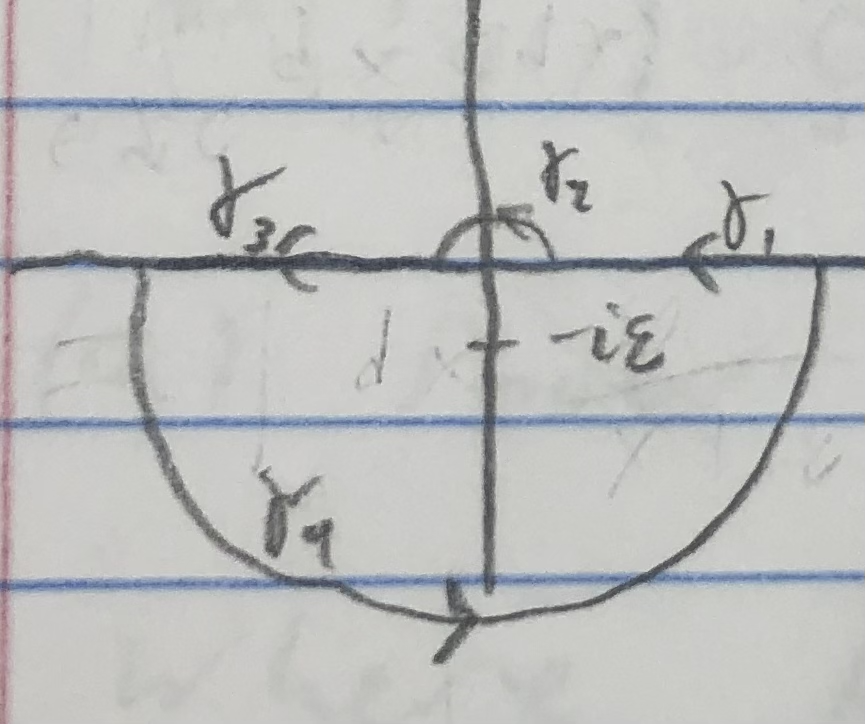
\includegraphics[scale=.2]{Images/contours}
    \caption{Contour for line integral}
    \label{fig:fig1}
\end{figure}


\hdashrule[0.5ex][c]{\linewidth}{0.5pt}{1.5mm}


\underline{Miscellaneous details between derivations}\\
\underline{Note:} $e^{-i \Delta_i t/\hbar} |i \rangle \implies e^{- i \Delta_i t/\hbar - i E_i t/\hbar} |i \rangle\\
\implies E_i \rightarrow E_i + \Delta_i$ as a result of perturbation\\
$\implies \Delta_i$ is the level shift of time dependent perturbation theory\\
\underline{recall:} $\frac{\dot{c}_i(t)}{c_i(t)} = - \frac{i}{\hbar} \Delta_i \approx - \frac{i}{\hbar}(V_{ii} + \sum_{m \neq i} \frac{| V_{mi}|^2}{E_i - E_m + i \hbar \eta})\\
\Delta_i = \Delta_i^{(1)} + \Delta_i^{(2)} + \cdots\\
\implies \Delta_i^{(1)} = V_{ii};\,\, \Delta_i^{(2)} = \sum_{m \neq i} \frac{|V_{mi}|^2}{E_i - E_m + i \hbar \eta}\\$
\underline{recall:} $\lim_{\epsilon \rightarrow 0} \frac{1}{x+ i \epsilon} = Pr \frac{1}{x}- i \pi \delta(x)\\
\implies \begin{cases} Re(\Delta_i^{(2)}) = Pr \sum_{m \neq i} \frac{|V_{mi}|^2}{E_i - Em}\\
Im(\Delta_i^{(2)}) = - \sum_{m \neq i} | V_{mi}|^2 \delta(E_i - E_m)
\end{cases}$
\underline{recall:} $\mathcal{W} = \frac{2 \pi}{\hbar} W_{fi}^2 \rho(E_{fi})\\
\rho(E_{fi}) \rightarrow \delta(E_n - E_i);\,\, W_{fi}^2 \rightarrow V_{ni}|^2\\
\implies \mathcal{W}_{i \rightarrow n} = \frac{2 \pi}{\hbar} |V_{ni}|^2 \delta(E_n - E_i)\\
\implies \sum_{m \neq i} \mathcal{W}_{i \rightarrow n} = \sum_{m \neq i} \frac{2 \pi}{\hbar} |V_{mi}|^2 \delta(E_n - E_i) = - \frac{2}{\hbar} Im[\delta_i^{(2)}]\\$
\underline{recall:} $e^{- i\Delta_it/\hbar} = c_i(t)\\
\implies c_it(t) = e^{- i ( Re(\Delta_i) + i Im(\Delta_i))t/\hbar} = e^{- i Re(\Delta_i) t/\hbar +Im(\Delta_i)t/\hbar}\\
|c_i|^2 = e^{2 Im(\Delta_i) t/\hbar} = e^{- \Gamma_it/\hbar}\\
\implies \frac{\Gamma_i}{\hbar} \equiv - \frac{2}{\hbar} Im(\Delta_i)$


\hdashrule[0.5ex][c]{\linewidth}{0.5pt}{1.5mm}


\item \underline{$Im(\Delta_i^{(2)}) = - \pi \sum_{m \neq i} |V_{mi}|^2 \delta(E_i - E_m)$}\\
\underline{recall:} $\lim_{\epsilon \rightarrow 0} \frac{1}{x+ i \epsilon} = Pr \frac{1}{x} - i \pi \delta(x);\,\, \Delta_i^{(2)} = \sum_{m \neq i} \frac{|V_{mi}|^2}{(E_i - E_m + i \hbar \eta)}\\$
\underline{Note:} Pr means principal value\\
$\implies \Delta_i^{(2)} = \sum_{m \neq i} |V_{mi}|^2 \lim_{\eta \rightarrow 0} \frac{1}{E_i- E_m + i \hbar \eta}\\
-= \sum_{m \neq i} |V_{mi}|^2 ( Pr \frac{1}{E_i - E_m} - i \pi \delta(E_i - E_m))\\
= \sum_{m \neq i} |V_{mi}|^2 Pr \frac{1}{E_i - E_m} - i \pi \sum_{m \neq i} |V_{mi}|^2 \delta( E_i - E_m)\\
= Re(\Delta_i^{(2)})+ i Im (\Delta_i^{(2)})\\
\therefore Im ( \Delta_i^{(2)}) = - \pi \sum_{m \neq i} |V_{mi}|^2 \delta(E_i - E_m)$


\hdashrule[0.5ex][c]{\linewidth}{0.5pt}{1.5mm}


\item \underline{$|c_i|^2 = e^{2 Im(\Delta_i)t/\hbar} = e^{-\Gamma_i t/\hbar} dt$}\\
\underline{recall:} $c_i(t) = e^{- i( Re(\Delta_i) + i Im(\Delta_i))t/\hbar} = e^{- i \Delta_it/\hbar}\\
\implies |c_i(t)|^2 = e^{2 Im(\Delta_i)t/\hbar}\\$
\underline{recall:} $\frac{\dot{c}_i(t)}{c_i(t)} = - \frac{i}{\hbar} \Delta_i = - \frac{i}{\hbar}( V_{ii} + \sum_{m\neq i} \frac{|V_{mi}|^2}{E_i - E_m + i \hbar \eta});\,\, \Delta_i = \Delta_i^{(1)} + \Delta_i^{(2)} + \cdots\\
\implies Im(\Delta_i) \approx Im( \Delta_i^{(2)}) \approx - \pi \sum_{m \neq i} |V_{mi}|^2 \delta(E_i - E_m)\\$
\underline{recall:} $\mathcal{W}_{i \rightarrow n} \approx \frac{2 \pi}{\hbar} |V_{ni}|^2 \delta(E_n - E_i)\\
\implies \sum_{m \neq i } \mathcal{W}_{i \rightarrow n} = \frac{2 \pi}{\hbar} \sum_{m \neq i} | V_{mi}|^2 \delta(E_i - E_m ) = - \frac{2}{\hbar} Im(\Delta_i^{(2)})\\
\therefore |c_i|^2 = e^{2 Im(\Delta_i)t/\hbar}\\
\implies \frac{\Gamma_i}{\hbar} \equiv - \frac{2}{\hbar} Im( \Delta_i)\\$
This also motivates defining the lifetime as $\frac{\hbar}{\Gamma_i} = \tau_i$


\hdashrule[0.5ex][c]{\linewidth}{0.5pt}{1.5mm}


\item \underline{$f(E) = \frac{\psi(0)}{E- [ E_i + Re(\Delta_i)]+ i \Gamma/2}$}\\
\underline{Note:} $|\psi \rangle = e^{- t/2 \tau_i} e^{-i Re(\Delta_i) t/\hbar} e^{- i E_i t/\hbar} | i \rangle; \tau_i = \frac{\hbar}{\Gamma_i}\\
\implies \psi(t) = e^{- \Gamma_i t/2 \hbar} e^{-i Re(\Delta_i) t/\hbar} e^{-i E_i t/\hbar} \psi(0)\\
\implies f(E) = \int dt \psi(t) e^{i E t/\hbar} = \int_0^{\infty} dt e^{[i ( E - [ E_i + Re(\Delta_i)]) - \Gamma_i/2]t/\hbar} \psi(0)\\
= \frac{- \psi(0)}{i(E- [ E_i + Re(\Delta_i)])- \Gamma_i/2}\\
= \frac{\psi(0)}{( E- [ E_i + Re(\Delta_i)]) + i \Gamma_i/2}\\
\therefore f(E) = \frac{\psi(0)}{(E- [E_i + Re(\Delta_i)]) + i \Gamma_i/2}$ (Breit-Wigner formula)\\
$f(E)$ is like the wave function in energy space, the probability that a particle will have energy $E$ is $|f(E)|^2$
 (I don't understand why there is only a half Fourier transform and also why it is missing the pre-factor)


\hdashrule[0.5ex][c]{\linewidth}{0.5pt}{1.5mm}


\item \underline{$\sigma = \frac{Number of scattering events}{\rho_A \ell_A \rho_B \ell_B A}$}\\
$\sigma$ tells us how often particles collide.\\
Assume we have a fixed bunch of particles $A$ which $\rho_A$, $\ell_A$; and $B$ with $\rho_B$, $\ell_B$. They share a common area $A$.\\
It makes sense that the number of scattering events is poroportional to all of these quantties\\
$\implies N \propto \rho_B \ell_A \rho_B \ell_B A$\\
the constant of proportionality is $\sigma\\
\therefore \sigma= \frac{N}{\rho_A \ell_A \rho_B \ell_B A}\\$


\hdashrule[0.5ex][c]{\linewidth}{0.5pt}{1.5mm}


\underline{Note:} the cross section tells us how often a specific process occurs, e.g. $e^+ e^- \rightarrow \mu^+ \mu^-\\$
$\sigma_{tot} = \sigma_{\mu^+ \mu^-} + \sigma_{\tau^+ \tau^-} + \cdots ?$\\


\hdashrule[0.5ex][c]{\linewidth}{0.5pt}{1.5mm}


\underline{Note:} we often care about not only the process but all the momentum of outgoing particle so $\sigma \rightarrow d \sigma$ (since we care about a very narrow range of momentum) so to make it finite we divide by $d^3 p_1 \cdots d^3 p_n$\\
$\implies \sigma \rightarrow \frac{d \sigma}{d^3p_1 \cdots d^3 p_n}$\\
integrate over $d^3 p_1 \cdots d^3 p_n$ to obtain how often a particle process happens with a certain range of outgoing momenta.\\


\hdashrule[0.5ex][c]{\linewidth}{0.5pt}{1.5mm}


\item \underline{ $\frac{d \sigma}{d^3 p_1 d^3 p_2} \rightarrow \frac{d \sigma}{d \Omega}$}\\
( assuming 2 species of outgoing particles we can integrate over the 4 constrained momentum components)\\
Lets prove that there are only 2 unconstrained momentum components.\\
right now we have 6 unconstrained components\\
$p_A^{\mu} + p_B^{\mu} = p_1^{\mu} + p_2^{\mu}\\$
A fixed $\implies \vec{p}_1 + \vec{p}_2 = \vec{p}_B \rightarrow \vec{p}_1 = \vec{p}_B - \vec{p}_2\\
\implies 3$ unconstrained components\\
$E_A + E_B = E_1 + E_2 = \sqrt{p_1^2 + m_1^2} + \sqrt{p_2^2 + m_2^2}\\
= \sqrt{p_1^2 + m_1^2} + \sqrt{(\vec{p}_B - \vec{p}_1)^2 + m_2^2}\\$
can solve for $| \vec{p}_1 | \implies 3 \rightarrow 2$ unconstrained components\\
we usually choose to parametrize these components by $\phi,\,\, \theta\\$


\hdashrule[0.5ex][c]{\linewidth}{0.5pt}{1.5mm}



\item \underline{$d \sigma = \frac{1}{2 E_A 2 E_B | v_A - v_B|} ( \Pi_f \frac{d^3 p_f}{(2 \pi)^3} \frac{1}{2 E_f}) 
\times | \mathcal{M}( p_A, p_B \rightarrow \{ p_f \} )|^2 (2 \pi)^4 \delta^{(4)} (p_A + p_B - \sum p_f)$}\\
\item \underline{$| \phi_A \phi_B \rangle_{in} = \int \frac{d^3 k_A}{(2 \pi)^3 \sqrt{2 E_A}} \phi_A( \vec{k}_{A}) | \vec{k}_A \rangle \int \frac{d^3 k_B}{(2 \pi)^3 \sqrt{2 E_B}} \phi_B ( \vec{k}_B) e^{- i \vec{b} \cdot \vec{k}_B} | \vec{k}_B \rangle$}\\
\underline{$out_\langle \phi_1 \phi_2 \cdots | = ( \Pi_f) \frac{d^3 p_f}{(2 \pi)^3} \frac{\phi_f(\vec{p}_f)}{\sqrt{2 E_f}} out_\langle \vec{p}_1 \vec{p}_2 \cdots |$}\\
\underline{recall:} $\langle \vec{x} | \vec{p} \rangle \propto e^{i \vec{p} \cdot \vec{x}}$ (single free particle $k$ state $\psi(x)$ from QM)\\
\underline{Note:} $|\vec{k} \rangle$ is a simultaneous eigenfunction of the free hamiltonian and the momentum operator
$\langle 0 | \phi( \vec{x}) | \vec{p} \rangle = e^{i \vec{p} \cdot \vec{x}}$ (allows us to interpret $\phi(\vec{x}) | 0 \rangle)\\$
\underline{recall:} $\phi( \vec{x}) = \int \frac{d^3 k}{(2 \pi)^3} e^{i \vec{k} \cdot \vec{x}} \phi(\vec{k})$\\
\underline{Note:} $|\phi \rangle \equiv \phi(x) | \vec{k} \rangle$ and not $| \phi \rangle = \phi(x) | 0 \rangle$; this makes sense because in order to obtain the wave function of a free field just hit it with $\langle 0|$\\
$\phi(\vec{x})$ is basically a particles field at $\vec{x}$ so $\phi(0)= \int \frac{d^3k}{(2 \pi)^3} \phi(\vec{k})$ is a particle's wave function evaluated at 0, also $\phi(\vec{x})$ as written from the fourier transform is centered at $\vec{x}'=0$\\
\underline{Note:} $\int \frac{d^3k}{(2 \pi)^3} | \phi( \vec{k})|^2=1 \implies \langle \phi | \phi \rangle = 1\\
\mathcal{P} = | \langle \phi_1 \phi_2 \cdots | \phi_A \phi_B \rangle |^2 \,\,$ 2 species initially (in) and n species finally (out)\\
$| \phi_A \phi_B \rangle_{in} = | \phi_A \rangle | \phi_B \rangle = \int \frac{d^3 k_A}{(2 \pi)^3 \sqrt{2 E_A}} \phi_A( \vec{k}_{A}) | \vec{k}_A \rangle \int \frac{d^3 k_B}{(2 \pi)^3 \sqrt{2 E_B}} \phi_B ( \vec{k}_B) e^{- i \vec{b} \cdot \vec{k}_B} | \vec{k}_B \rangle\\$
\underline{Note:} the previous line we evaluated $| \phi_A \rangle at \vec{x}=0$, (it seems like we only care about the transverse direction for some reason??) however, for $|\phi_B \rangle$ we still evaluate it at $\vec{x}=0$ but we had to shift it, that is $\phi(x) \rightarrow \phi'(x)=\phi(x-b)$ so for $x=0$ we have $\phi(-b)$ which explains the phase factor\\
$=\int \frac{d^3 k_A}{(2 \pi)^3} \int \frac{d^3 k_B}{(2 \pi)^3} \frac{\phi_A( \vec{k}_A) \phi_B( \vec{k}_B) e^{- i \vec{b} \cdot \vec{k}_B}}{\sqrt{(2 E_A)(2 E_B)}} | \vec{k}_A \vec{k}_B \rangle\\$
We could write\\
$out_\langle \phi_1 \phi_2 \cdots | = ( \Pi_f) \frac{d^3 p_f}{(2 \pi)^3} \frac{\phi_f(\vec{p}_f)}{\sqrt{2 E_f}} out_\langle \vec{p}_1 \vec{p}_2 \cdots |\\$


\hdashrule[0.5ex][c]{\linewidth}{0.5pt}{1.5mm}


\item \underline{$\mathcal{P} (AB \rightarrow 1\, 2 \cdots n)= \Pi_f \frac{d^3 p_f}{(2 \pi)^3} \frac{1}{2E_f} | {out}_\langle p_1 p_2 \cdots | \phi_A \phi_B \rangle |^2$}\\
\underline{recall:} $| \vec{p}(t) \rangle = e^{i H t} | \vec{p} \rangle\\
| \vec{k} \rangle \sim - T,\,\, | \vec{p} \rangle \sim - T\\
\implies {\rm{out}}_\langle \vec{p}_1 \vec{p}_2 \cdots | \vec{k}_A \vec{k}_B \rangle_{in}= \lim_{T \rightarrow \infty} \langle \vec{p}_1 \vec{p}_2 \cdots | \vec{k}_A \vec{k}_B \rangle = \lim_{T \rightarrow \infty} \langle \vec{p}_1 \vec{p}_2 \cdots | e^{- i H(2 T)} | \vec{k}_As \vec{k}_B \rangle\\
\implies {out}_\langle \vec{p}_1 \vec{p}_2 \cdots | \vec{k}_A \vec{k}_B \rangle_{in} \equiv \langle \vec{p}_1 \vec{p}_2 | S | \vec{k}_A \vec{k}_B \rangle\\
S = 1 + i T\\$
define $\langle \vec{p}_1 \vec{p}_2 \cdots | i T | \vec{k}_A \vec{k}_B \rangle = (2 \pi)^4 \delta^{(4)} ( k_A + k_B - \sum p_f) \cdot i M(k_A, k_B \rightarrow p_f)\\
M \sim f$ ($f$ from QM)\\
\underline{recall:} $out_\langle \phi_1 \phi_2 \cdots | = ( \Pi_f \int \frac{d^3 p_f}{(2 \pi)^3} \frac{\phi_f(\vec{p}_f)}{\sqrt{2 E_f}} out_\langle p_1 p_2 \cdots |\\
\mathcal{P} (AB \rightarrow 1\, 2 \cdots n)= | \langle \phi_1 \phi_2 \cdots | \phi_A \phi_B \rangle|^2\\
= | \Pi_f \int \frac{d^3 p_f}{(2 \pi)^3} \frac{\phi_f(\vec{p}_f)}{2 E_f} out_\langle p_1 p_2 \cdots | \phi_A \phi_B \rangle_{in}|^2\\
= \Pi_f \int \frac{d^3 p_f}{(2 \pi)^3 (2 E_f)} \Pi_{f'} \left [ \int \frac{d^3 p_{f'} | \phi_{f'} (p_{f'})|^2}{(2 \pi)^3 (2 E_f)} \right ] | \langle p_1 \cdots | \phi_A \phi_B \rangle |^2\\$
(the last line requires just a little bit of thought)\\
$
= \Pi_f \frac{d^3 p_f}{(2 \pi)^3} \frac{1}{2E_f} | {out}_\langle p_1 p_2 \cdots | \phi_A \phi_B \rangle |^2\\$
I think the reason $\phi_f( \vec{p}_f)$ disappears is due to $\int \frac{d^3k}{(2 \pi)^3} | \phi(\vec{k})|^2=1$\\


\hdashrule[0.5ex][c]{\linewidth}{0.5pt}{1.5mm}

\item \underline{$d \sigma = ( \Pi_f \frac{d^3 p_f}{(2 \pi)^3} \frac{1}{2 E_f}) ( \Pi_{i= A, B} \int \frac{d^3 k_i}{(2 \pi)^3} \frac{\phi_i( \vec{k}_i)}{\sqrt{2 E_i}} \int \frac{d^3 \bar{k}_i}{(2 \pi)^3} \frac{\phi_i^*( \bar{\vec{k}}_i)}{\sqrt{2 \bar{E}_i}}) (2 \pi)^2 \delta^{(2)} (k_B^{\perp} - \bar{k}_B^{\perp})$}
$\left [i \mathcal{M} ( \{ k_i \} \rightarrow \{ p_f \}) (2 \pi)^4 \delta^{(4)}( \sum k_i - \sum p_f) \right ]\\
\left [- i \mathcal{M}^* ( \{ \bar{k}_i\} \rightarrow \{ p_f \}) ( 2 \pi)^4 \delta^{(4)}(\sum \bar{k}_i - \sum p_f) \right ]$\\
single A many B\\
$N= \sum_{\text{all inident particles i}} \mathcal{P}_i = \int d^2 b n_B \mathcal{P}(\vec{b})\\
\vec{b} \sim$ impact parameter,\,\, $n_B \sim$ particles/unit area\\
$n_B$ constant roughly (over the effects of $\phi_A$)\\
$\implies \sigma = \frac{\text{Number of scatter events}}{\rho_A \ell_A \rho_B \ell_B A} = \frac{N}{n_B N_A} = \frac{N}{n_B \cdot 1} = \int d^2 b \mathcal{P}(\vec{b})\\
\implies d \sigma = \int d^2 b | \langle \phi_1 \phi_2 \cdots | \phi_A \phi_B \rangle |^2\\
= \int d^2 b ( \Pi_f \frac{d^3 p_f}{(2 \pi)^3} \frac{1}{2 E_f} ) | out_\langle p_1 \cdots p_n | \phi_A \phi_B \rangle_{in}|^2\\
= \int d^2 b ( \Pi_f \frac{d^3 p_f}{(2 \pi)^3} \frac{1}{2 E_f}) \langle p_1 \cdots p_n | \phi_A \phi_B \rangle \langle \phi_A \phi_B | p_1 \cdots p_n \rangle\\
= \int d^2 b ( \Pi_f \frac{d^3 p_f}{(2 \pi)^3} \frac{1}{2 E_f}) ( \Pi_{i= A, B} \int \frac{d^3 k_i}{(2 \pi)^3} \frac{\phi_i(\vec {k}_i)}{\sqrt{2 E_i}} \int \frac{d^3 \bar{k}_i}{(2 \pi)^3} \frac{\phi_i^* ( \bar{k}_i)}{\sqrt{2 \bar{E}_i}})\\
\times e^{i \vec{b} \cdot( \bar{\vec{k}}_B - \vec{k}_B) }( out_\langle \{ \vec{p}_f \} | \{\vec{k}_i \} \rangle_{in})( out_\langle \{ \vec{p}_f \} | \{ \bar{k}_i \} \rangle_{in})^*\\$
where $\langle \vec{p}_1 \cdots \vec{p}_n | \vec{k}_A \vec{k}_B \rangle_{in} \equiv \langle \{ \vec{p} \}_f| \{ \vec{k}_i \} \rangle_{in}?\\
\int d^2 b e^{i \vec{b} \cdot( \bar{\vec{k}}_B - \vec{k}_B)} = ( 2 \pi)^2 \delta^{(2)} ( \vec{k}_B^{\perp} - \bar{\vec{k}}_B^{\perp})\\
(out_\langle \{ p_f \} | \{ k_i \} \rangle_{in}) = i \mathcal{M}( \{k_i \} \rightarrow \{ p_f \} )( 2 \pi)^4 \delta^{(4)} ( \sum_i k_i - \sum_f p_f)\\
(out_\langle \{ p_f \} | \{ \bar{k}_i\} \rangle_{in})^* = - i \mathcal{M}^*( \{ \bar{k}_i \} \rightarrow \{p_f \}) ( 2 \pi)^4 \delta^{(4)}( \sum \bar{k}_i - \sum p_f)\\$
$x,y$ transverse, $z$ parallel to beam\\
$\implies d \sigma = ( \Pi_f \frac{d^3 p_f}{(2 \pi)^3} \frac{1}{2 E_f}) ( \Pi_{i= A, B} \int \frac{d^3 k_i}{(2 \pi)^3} \frac{\phi_i( \vec{k}_i)}{\sqrt{2 E_i}} \int \frac{d^3 \bar{k}_i}{(2 \pi)^3} \frac{\phi_i^*( \bar{\vec{k}}_i)}{\sqrt{2 \bar{E}_i}}) (2 \pi)^2 \delta^{(2)} (k_B^{\perp} - \bar{k}_B^{\perp})
\left [i \mathcal{M} ( \{ k_i \} \rightarrow \{ p_f \}) (2 \pi)^4 \delta^{(4)}( \sum k_i - \sum p_f) \right ]\\
\left [- i \mathcal{M}^* ( \{ \bar{k}_i\} \rightarrow \{ p_f \}) ( 2 \pi)^4 \delta^{(4)}(\sum \bar{k}_i - \sum p_f) \right ]\\$



\hdashrule[0.5ex][c]{\linewidth}{0.5pt}{1.5mm}


\item \underline{$\int d^3 \bar{k}_A \phi_A^* (\bar{k}_A) \int d^3 \bar{k}_B \phi_B^* (\bar{k}_b) \delta^{(4)} ( \sum_i \bar{k}_i - \sum p_f) \delta^{(2)} (k^{\perp}_B - \bar{k}^{\perp}_B) \delta^{(4)} ( \sum_i k_i - \sum p_f)$}\\
\underline{$= \delta^{(4)} ( \sum_i k_i - \sum_f p_f) \phi_A^*( k_A ) \phi^*_B ( k_B) \frac{1}{|\frac{k_A^z}{E_A} - \frac{k_B^z}{E_B}|}$}\\
$\int d^3 \bar{k}_A \phi_A^* (\bar{k}_A) \int d^3 \bar{k}_B \phi_B^* (\bar{k}_b) \delta^{(4)} ( \sum_i \bar{k}_i - \sum p_f) \delta^{(2)} (k^{\perp}_B - \bar{k}^{\perp}_B) \delta^{(4)} ( \sum_i k_i - \sum p_f)\\
= \int d^3 \bar{k}_A \phi_A^* (\bar{k}_A) \int d \bar{k}_B^z \phi_B^* (k_B^{\perp}, \bar{k}_B^z) \delta^{(4)} (\sum_i \bar{k}_i - \sum p_f) \delta^{(4)} ( \sum_i k_i - \sum p_f)\\
\underline{recall:} \delta(x-y) \delta(z-y) = \delta(x-y) \delta(z-x)\\
x= \sum_i k_i;\,\, y = \sum_f p_f;\,\, z= \sum_i \bar{k}_i\\
\implies \delta^{(4)} ( \sum_i \bar{k}_i - \sum p_f ) \delta^{(4)} ( \sum_i k_i - \sum p_f)\\
= \delta^{(4)} ( \sum_i k_i - \sum_f p_f) \delta^{(4)} ( \sum_i \bar{k}_i - \sum_i k_i)\\$
insert into previous\\
$\implies \delta^{(4)} ( \sum_i k_i - \sum_f p_f)\\
\int d^3 \bar{k}_A \phi( \bar{k}_A) \int d \bar{k}_B^z \phi^*_B( k_B^{\perp}, \bar{k}_B^z)\\
\delta^{(2)}( \bar{k}_A^{\perp} + k_B^{\perp} - k_A^{\perp} - k_B^{\perp}) \delta ( \bar{k}_A^z + \bar{k}_B^z - k_A^z - k_B^z) \delta(\bar{E}_A + \bar{E}_B - E_A - E_B)\\
= \delta^{(4)} ( \sum_i k_i - \sum_F p_f)\\
\int d \bar{k}_A^z \phi^*_A ( k_A^{\perp}, \bar{k}_A^z) \int d \bar{k}_B^z \phi^* (k_B^{\perp} , \bar{k}_B^z)\\
\delta( \bar{k}_A^z + \bar{k}_B^z - k_A^z - k_B^z) \delta ( \bar{E}_A + \bar{E}_B - E_A - E_B)\\
= \delta^{(4)} ( \sum_i k_i - \sum_f p_f) \int d \bar{k}_A^z \phi_A^* ( k_A^{\perp}, \bar{k}_A^z \phi^*_B ( k_B^{\perp} , \bar{k}_B^z)_{\bar{k}_B^z= \sim}\\
\delta( \sqrt{k^{\perp 2}_A + m_A^2 + \bar{k}_A^{z 2}} + \sqrt{k_B^{\perp 2} + ( k_A^z - \bar{k}_A^z + k_B^z )^2 + m_B^2} - E_A - E_B)\\
\delta( f(\bar{k}_A^z))$ has a zero where $\bar{k}_A^z = k_A^z \implies \bar{k}_B^z = k_B^z\\
= \delta^{(4)} ( \sum_i k_i - \sum_f p_f) \phi_A^*( k_A ) \phi^*_B ( k_B) \frac{1}{|\frac{k_A^z}{E_A} - \frac{k_B^z}{E_B}|}\\$
\underline{Note:} We used $\int dx \delta( f(x)) \phi(x) = \sum_j \frac{1}{|f'(x_j)|} \phi( x_j)\\$
and $\frac{\bar{k}_A^z}{\bar{E}_A} - \frac{\bar{k}_B^z}{\bar{E}_B} = \frac{k_A^z}{E_A} - \frac{k_B^z}{E_B}$ due to all of the constraints.
\\
\\
\\
$ \frac{1}{| \frac{\bar{k}_A^z}{\bar{E}_A} - \frac{\bar{k}_B^z}{\bar{E}_B}|} \equiv \frac{1}{|v_A - v_B|} \\
\frac{\bar{k}_A^z}{\bar{E}_A} \sim \frac{p}{E} = \frac{\gamma m v}{\gamma m} =v\\$
initial wave packets highly localized around $\vec{p}_A, \vec{p}_B$ which I believe allows us to pull the amplitude out of the integral
$\implies d \sigma = ( \Pi_f \frac{d^3 p_f}{(2 \pi)^3} \frac{1}{2 E_f}) ( \Pi_{i= A, B} \int \frac{d^3 k_i}{(2 \pi)^3} \frac{\phi_i( \vec{k}_i)}{\sqrt{2 E_i}} \int \frac{d^3 \bar{k}_i}{(2 \pi)^3} \frac{\phi_i^*( \bar{\vec{k}}_i)}{\sqrt{2 \bar{E}_i}}) (2 \pi)^2 \delta^{(2)} (k_B^{\perp} - \bar{k}_B^{\perp})
\left [i \mathcal{M} ( \{ k_i \} \rightarrow \{ p_f \}) (2 \pi)^4 \delta^{(4)}( \sum k_i - \sum p_f) \right ]\\
\left [- i \mathcal{M}^* ( \{ \bar{k}_i\} \rightarrow \{ p_f \}) ( 2 \pi)^4 \delta^{(4)}(\sum \bar{k}_i - \sum p_f) \right ]\\
= ( \Pi_f \frac{d^3 p_f}{(2 \pi)^3} \frac{1}{2 E_f}) \frac{| \mathcal{M}( p_A, p_B \rightarrow \{ p_f \})|^2}{2 E_A 2 E_B | v_A - v_B|} \int \frac{d^3 k_A}{(2 \pi)^3} \int \frac{d^3 k_B}{(2 \pi)^3}\\
\times | \phi_A ( \vec{k}_A)|^2 | \phi_B ( \vec{k}_B)|^2 (2 \pi)^4 \delta^{(4)} ( k_A + k_B - \sum p_f)\\$
this is main result we just need to go to the center of mass frame\\

\hdashrule[0.5ex][c]{\linewidth}{0.5pt}{1.5mm}


\item \underline{improve this part}
$\int d \bar{k}_A^z d \bar{k}_B^z \delta(\bar{k}_A^z + \bar{k}_B^z - \sum p_f^z) \delta( \bar{E}_A + \bar{E}_B - \sum E_f)\\
= \int d \bar{k}_A^z \delta( \bar{E}_A + \bar{E}_B - \sum E_f)|_{\bar{k}_B^z = \sum p_f^z - \bar{k}_A^z}\\
= \int d \bar{k}_A^z \delta( \sqrt{\bar{k}_A^2 + m_A^2} + \sqrt{ \bar{k}_B^2 + m_B^2} - \sum E_f)|_{\bar{k}_B^z = \sum p^z_f - \bar{k}_A^z}\\
= \frac{1}{| \frac{\bar{k}_A^z}{\bar{E}_A} - \frac{\bar{k}_B^z}{\bar{E}_B}|} \equiv \frac{1}{|v_A - v_B|} (???)\\
\frac{\bar{k}_A^z}{\bar{E}_A} \sim \frac{p}{E} = \frac{\gamma m v}{\gamma m} =v\\$
initial wave packets highly localized around $\vec{p}_A, \vec{p}_B$\\
needs more steps here, the fact that one integral pops up has to deal with the factor of $e^{-ib k}$ and the integral turning into a delta function\\
$\implies d \sigma = ( \Pi_f \frac{d^3 p_f}{(2 \pi)^3} \frac{1}{2 E_f}) \frac{| \mathcal{M}( p_A, p_B \rightarrow \{ p_f \})|^2}{2 E_A 2 E_B | v_A - v_B|} \int \frac{d^3 k_A}{(2 \pi)^3} \int \frac{d^3 k_B}{(2 \pi)^3}\\
\times | \phi_A ( \vec{k}_A)|^2 | \phi_B ( \vec{k}_B)|^2 (2 \pi)^4 \delta^{(4)} ( k_A + k_B - \sum p_f)\\$
this is main result we just need to go to the center of mass frame\\


\hdashrule[0.5ex][c]{\linewidth}{0.5pt}{1.5mm}


\item \underline{$( \frac{d \sigma}{d \Omega})_{CM} = \frac{1}{2 E_A 2 E_B | v_A - v_B |} \frac{| \vec{p}_1 |}{(2 \pi)^4 4 E_{CM}} | \mathcal{M}( p_A, p_B \rightarrow p_1, p_2)|^2$}\\
$k_A + k_B \sim p_A + p_B \implies$ take $\delta$ out of integral\\
and we have\\
$( \int \frac{ d^3 k_A}{(2 \pi)^3} | \phi_A( \vec{k}_A)|^2 )( \int \frac{d^3 k_B}{(2 \pi)^3} | \phi_B ( \vec{k}_B)|^2 ) \approx 1\\
\implies d \sigma = \frac{1}{2 E_A 2 E_B | v_A - v_B|} ( \Pi_f \frac{d^3 p_f}{(2 \pi)^3} \frac{1}{2 E_f})\\
\times \mathcal{M}( p_a, p_B \rightarrow \{ p_f \} ) |^2 ( 2 \pi)^4 \delta^{(4)} ( p_A + p_B - \sum p_f)\\$
everything except $\frac{1}{2 E_A 2 E_B | v_A - v_B|}$ is Lorentz invariant\\
$E_A E_B | v_A - v_B| = |E_A v_A E_B - E_A E_B v_B|= | p_A^z E_B - E_A p_B^z|\\$
since $E_A v_a = \gamma m_A v_A = p_A^z$ since $v_A$ is in $z$ direction\\
$\implies \frac{1}{E_A E_B | v_A - v_B|} = \frac{1}{|E_B p_A^z - E_A p_B^z|} = \frac{1}{| \epsilon_{\mu x y \nu} p_A^{\mu} p_{B}^{\nu}|}\\
\int d \Pi_n = ( \Pi_f \int \frac{d^3 p_f}{(2 \pi)^3} \frac{1}{2 E_f})( 2 \pi)^4 \delta^{(4)} ( p_A + p_B - p_1 - p_2)\\
= ( \int \frac{d^3 p_1}{(2 \pi)^3} \frac{1}{2 E_1})( \sum \frac{d^3 p_2}{(2 \pi)^3} \frac{1}{2 E_2}( 2 \pi)^4 \delta^{(4)}( p_A + p_B - p_1 - p_2))\\
= \int \frac{d^3 p_1}{( 2\pi)^3 2 E_1 2 E_2} (2 \pi) \delta( E_A + E_B - p_1 - p_2)\\$
COM,$\,\, E_{CM} = E_A + E_B;\,\, \vec{p}_2 =- \vec{p}_1\\
\implies \int \frac{ dp_1 p_1^2 d \Omega}{(2 \pi)^3 2 E_1 2 E_2} (2 \pi) \delta( E_{cm} - E_1 - E_2)\\$
\underline{recall:} $\int dx \delta[ f(x)] \phi(x) = \frac{1}{|f'(x)|} \phi(x)\\
\implies \int d \Pi_2 = \int \frac{d \Omega}{(2 \pi)^3 2 E_1 2 E_2} ( 2 \pi) \int d p_1 p_1^2 \delta( E_{cm} - \sqrt{p_1^2 + m_1^2} - \sqrt{p_1^2 + m_2^2})\\
\phi(p_1) = p_1^2,\,\, f(p_1) = E_{cm} - \sqrt{p_1^2 + m_1^2} - \sqrt{p_1^2 + m_2^2}\\
\implies f'(p_1) = - \frac{p_1}{E_1} - \frac{p_1}{E_2}\\
\implies \int d \Pi_2 = \int \frac{d \Omega}{(2 \pi)^3 2 E_1 2 E_2} ( 2 \pi) ( p_1^2 |( \frac{p_1}{E_1} + \frac{p_1}{E_2})^{-1}|)\\
= \int d \Omega \frac{1}{16 \pi^2} \frac{1}{E_1 E_2} p_1^2 |( \frac{E_2 p_1 + p_1 E_1}{E_1 E_2})^{-1}|\\
= \int d \Omega \frac{1}{16 \pi^2} | \frac{1}{E_2 p_1 + p_1 E_1}| p_1^2\\
= \int d \Omega \frac{1}{16 \pi^2} \frac{1}{E_{CM}} | \vec{p}_1|\\$
Notice $\int d \Omega$ cant be performed, why?\\ 
integrate out $\phi$, since we can assume reaction takes place in a plane.\\
$\implies \int d \Pi_2 = \int d \cos \theta \frac{1}{16 \pi} \frac{2 | \vec{p}_1|}{ E_{CM}}$ (not important right now)\\
$\implies d \sigma = \frac{1}{2 E_A 2 E_B | v_A - v_B|} \frac{d \Omega| \vec{p}_1|}{(2 \pi)^2 4 E_{CM}} | \mathcal{M}( p_A, p_B \rightarrow p_1, p_2)|^2\\
\therefore ( \frac{d \sigma}{d \Omega})_{CM} = \frac{1}{2 E_A 2 E_B | v_A- v_B|} \frac{|\vec{p}_1|}{(2 \pi)^2 4 E_{CM}} | \mathcal{M}(p_A, p_B \rightarrow p_1, p_2)|^2\\
$

\hdashrule[0.5ex][c]{\linewidth}{0.5pt}{1.5mm}


\item \underline{$( \frac{d \sigma}{d \Omega})_{CM}= \frac{|M|^2}{64 \pi^2 E_{cm}^2}$} (all four masses equal)\\
\underline{recall:} $( \frac{d \sigma}{d \Omega})_{CM} = \frac{1}{2 E_A 2 E_B | v_A - v_B|} \frac{| \vec{p}_1|}{(2 \pi)^2 4 E_{CM}} | \mathcal{M}(p_A, p_B \rightarrow p_1, p_2 ) |^2\\
m \rightarrow 0,\,\,$ all four masses equal\\
$| v_A - v_B| = 2,\,\, E_A = E_B = \frac{1}{2} E_{CM};\,\, |\vec{p}_1| = \gamma m= E_1 = \frac{E_{CM}}{2}\\
\implies ( \frac{d \sigma}{d \Omega})_{CM} = \frac{1}{2 E_{CM}^2} \frac{E_{CM}}{2 ( 2 \pi)^2 4 E_{CM}} |M|^2\\
= \frac{|M|^2}{ 64 \pi^2 E_{CM}^2}$


\hdashrule[0.5ex][c]{\linewidth}{0.5pt}{1.5mm}


\item \underline{$\int d\bar{k}_A^z \delta( \sqrt{ \bar{k}_A^2 + m_A^2 } + \sqrt{ \bar{k}_B^2 + m_B^2} - \sum E_f)|_{\bar{k}_B^z = \sum p_f^z - \bar{k}_A^z}= \frac{1}{|v_A -v_B|}$}\\
\underline{recall:} $\int d x \delta [ f(x)] \phi(x) = \sum_j \frac{1}{|f'(x_j)|} \phi(x_j)$ $x_j$ are roots of the function f\
$f(k_A^z) = \sqrt{ \bar{k}_A^2 + m_A^2} + \sqrt{ \bar{k}_B^2 + m_B^2} - \sum E_f\\
= \sqrt{ ({\bar{k}_A^{\perp}})^2 + ({\bar{k}_A^z})^2 + m_A^2} + \sqrt{ ( \sum p_f^z - k_A^z)^2 + (\bar{k}_B^{\perp})^2 + m_B^2} - \sum E_f\\
\implies f'(k_A^z) = \frac{\bar{k}_A^z}{\sqrt{\bar{k}_A^2 + m_A^2}} - \frac{( \sum p_f^z - k_A^z)}{\sqrt{ \bar{k}_B^2 + m_B^2}}\\
= \frac{\bar{k}_A^z}{E_A} - \frac{\bar{k}_B^z}{E_B}\\
\frac{\bar{k}_A^z}{E_A} \sim \frac{p}{E} \sim \frac{\gamma m v}{\gamma m} \sim v\\
= v_A - v_B\\
\therefore \int d \bar{k}_A^z \delta( \sqrt{\bar{k}_A^2 + m_A^2} + \sqrt{ \bar{k}_B^2 + m_B^2} - \sum E_f)|_{\bar{k}_B^z = \sum p_f^z -\bar{k}_A^z}\\
= \frac{1}{|v_A - v_B|}$


\underline{Note:} $\Gamma = \frac{\text{Number of decays per unit time}}{\text{Number of A particles present}}$\\
We assume $A$ is at rest\\
understand $\frac{d \sigma}{d \Omega} = |f|^2$ next\\


\hdashrule[0.5ex][c]{\linewidth}{0.5pt}{1.5mm}


\item \underline{$d \Gamma = \frac{1}{2 m_A} ( \Pi_f \frac{d^3 p_f}{(2 \pi)^3} \frac{1}{2 E_f}) ( \mathcal{M}( m_A \rightarrow \{ p_f \} ) |^2 (2 \pi)^4 \delta^{(4)} (p_A - \sum p_f)$}\\
\underline{recall:} $\frac{1}{2 E_A 2 E_B | v_A - v_B|} ( \Pi_f \frac{d^3 p_f}{(2 \pi)^3} \frac{1}{2 E_f})\\
\times | \mathcal{M}( p_A, p_B \rightarrow \{ p_f \} |^2 (2 \pi)^4 \delta^{(4)} (p_A + p_B - \sum p_f) = d \sigma\\$
remove factors that don't make sense for a one body decay\\
$\implies d \Gamma = \frac{1}{2 m_A} ( \Pi_f \frac{d^3 p_f}{(2 \pi)^3} \frac{1}{2 E_f}) \times | \mathcal{M}( m_A \rightarrow \{ p_f \})|^2 (2 \pi)^4 \delta^{(4)}( p_A - \sum p_f)$


\hdashrule[0.5ex][c]{\linewidth}{0.5pt}{1.5mm}


\item \underline{$\hat{U}_I(t',t) = T \exp(- i \int_t^{t'} d \tau H_{int}^I(\tau))$}\\
\underline{Note:} $e^{i H_0 \Delta} e^{- i H \Delta} = e^{i(H_0 - H) \Delta + O(\Delta^2)} \approx e^{- i H_I(t) \Delta}\\
\hat{U}_I(t',t) = \hat{U}(t', t'- \Delta) \hat{U}(t'- \Delta, t'- 2 \Delta) \cdots \hat{U}(t + \Delta, t)\\
= e^{- i H_{int}^I(t'- \Delta)\Delta} \cdot e^{- i H_{int}^I (t' - 2 \Delta) \Delta} \cdots e^{- i H_{int}^I(t) \Delta}\\
= T e^{- i H_{int}^I (t'- \Delta) \Delta} \cdot e^{- i H_{int}^I(t'-2 \Delta) \Delta} \cdots e^{- i H_{int}^I(t) \Delta}\\
= T^{- i i H_{int}^I(t'- \Delta) \Delta - i H_{int}^I(t' - 2 \Delta) \Delta- \cdots - i H_{int}^I(t) \Delta}\\
= T \exp \left ( - i \int_t^{t'} d \tau H_{int}^I(\tau) \right )\\$


\hdashrule[0.5ex][c]{\linewidth}{0.5pt}{1.5mm}


\item \underline{$U_I(t + \Delta,t) = e^{- i H_{int}^I(t) \Delta}$}\\
\underline{recall:} $U_I(t',t) = e^{i H_0 t'} e^{- i H(t'- t)} e^{- i H_0 t}\\
\implies U_I(t + \Delta, t) = e^{i H_0 ( t + \Delta)} e^{- i H( \Delta} e^{- i H_0 t}\\
= e^{i H_0 t} e^{i H_0 \Delta} e^{- i H \Delta} e^{- i H_0 t}= e^{i H_0 t} e^{- i H_I(t) \Delta} e^{- i H_0 t}\\$
expand $e^{- i H \Delta}$ and Note $e^{i H_0} H^n e^{- i H_0 t} = e^{i H_0 t} H e^{- i H_0 t} e^{i H_0 t} H \cdots\\
= H_I^n\\
\implies U_I(t + \Delta, t) = e^{- i H_{int}^I(t) \Delta}\\$


\hdashrule[0.5ex][c]{\linewidth}{0.5pt}{1.5mm}


$\mathcal{L}_I = - \frac{\lambda}{4 !} \phi^4 \implies \hat{\mathcal{H}}_I = \frac{\lambda}{4!} \hat{\phi}(x)^4$


\hdashrule[0.5ex][c]{\linewidth}{0.5pt}{1.5mm}


$\implies \hat{S} = T [ \exp( - i \int d^4 z \hat{\mathcal{H}}_I(z))]\\
= T[ 1- i \int d^4 z \hat{\mathcal{H}}_I(z) + \frac{(-i)^2}{2} \int d^4 y d^4 w \hat{\mathcal{H}}_I(y) \hat{\mathcal{H}}_I(w) + \cdots ]\\
= T [ 1- \frac{i \lambda}{4 !} \int d^4 z \hat{\phi}(z)^4 + \frac{(- i)^2}{2!} ( \frac{\lambda}{4!})^2 \int d^4 y d^4 w \hat{\phi}(y)^4 \hat{\phi}(w)^4 + \cdots ]\\$


\hdashrule[0.5ex][c]{\linewidth}{0.5pt}{1.5mm}


$A = \langle q | \hat{S} | p \rangle = ( 2 \pi)^3 ( 2E_q)^{1/2} ( 2 E_p)^{1/2} T[ \langle 0 | \hat{a}_q \hat{a}_p^{\dagger} | 0 \rangle + ( \frac{- i \lambda}{4}) \int d^4 \langle 0 | \hat{a}_q \hat{\phi}(z)^4 \hat{a}_p^{\dagger} | 0 \rangle + \frac{(- i)^2}{2 !} ( \frac{\lambda}{4!})^2 \int d^4 y d^y w \hat{\phi}(y)^4 \hat{\phi}(w)^4 + \cdots ]\\$


\hdashrule[0.5ex][c]{\linewidth}{0.5pt}{1.5mm}


\item \underline{$A^{(1)} = - \frac{i \lambda}{4!} \int d^4 z [ 3 \langle 0 | \hat{a}_q \hat{a}_p^{\dagger} | 0 \rangle \langle 0 | \hat{\phi}(z) \hat{\phi}(z) | 0 \rangle \langle 0 | \hat{\phi}(z) \hat{\phi}(z) | 0 \rangle$}\\
\underline{$+ 12 \langle 0 | \hat{a}_q \hat{\phi}(z) | 0 \rangle \langle 0 | \hat{\phi}(z) \hat{\phi}(z) | 0 \rangle \langle 0 | \hat{\phi}(z) \hat{a}_p^{\dagger} | 0 \rangle$}\\
use wicks theorem on $T \langle 0 | \hat{a}_q \hat{\phi}(z)^4 \hat{a}_p^{\dagger} | 0 \rangle\\$
\underline{recall:} $T[ \hat{A} \hat{B} \cdots \hat{Z} ] = N [ \hat{A} \hat{B} \hat{C} \cdots \hat{Z}$ + all possible contractions of $\hat{A} \hat{B} \cdots \hat{Z} ]\\$
\underline{Note:} $\langle 0 | N[ \hat{a}_q \hat{\phi} (z)^4 \hat{a}_p^{\dagger} ] | 0 \rangle = 0\\$
there will be two types of contractions, first is kinds like \\
$\wick{\langle 0 | \c1 a_q \c2 \phi \c2 \phi \c3 \phi \c3 \phi \c1 a_p^{\dagger} | 0 \rangle}\\
= \langle n | \hat{a}_q\hat{a}_p^{\dagger} | 0 \rangle \langle 0 | \hat{\phi} \hat{\phi} | 0 \rangle \langle 0 | \hat{\phi} \hat{\phi} | 0 \rangle$
there are 3 of these contractions since we can choose 3 other phi's to contract phi with, and there is only one way to contract the a's.\\
the other term is like\\
$\wick{\langle 0 | \c1 a_q \c1 \phi \c2 \phi \c2 \phi \c3 \phi \c3 a_p^{\dagger} | 0 \rangle} = \langle 0 | a_q \phi | 0 \rangle \langle 0 | \phi \phi | 0 \rangle \langle 0 | \phi a_p^{\dagger} | 0 \rangle\\$
does $\langle 0 | N[ a_q a_p^{\dagger} ] | 0 \rangle = 0?\\$
there are 12 ways this contraction can happen, four choices of $\phi$ to contract $a_q$ with and 3 choices of $\phi$ to contract $a_p^{\dagger}$ with.\\
$\implies A^{(1)} = - \frac{i \lambda}{4 !} \int d^4 z [ 3 \langle 0 | a_q a_p^{\dagger} | 0 \rangle \langle 0 | \phi \phi | 0 \rangle \langle 0 | \phi \phi | 0 \rangle + 12 \langle 0 | a_q \phi | 0 \rangle \langle 0 |  \phi \phi | 0 \rangle \langle 0 | \phi a_p^{\dagger} | 0 \rangle ]$


\hdashrule[0.5ex][c]{\linewidth}{0.5pt}{1.5mm}


\underline{Note:}$A = A^{(0)} + A^{(1)} + A^{(2)} + \cdots\\$
\underline{Note:} $\wick{  \c1 \phi(y) \c1 \phi(z) } = \langle 0 | T \hat{\phi}(y) \hat{\phi}^{\dagger}(z) | 0 \rangle= \Delta( y- z)$\\
\underline{Note:} $\hat{\phi}^{\dagger} = \hat{\phi},\,\, \hat{\phi}$ is real here 


\hdashrule[0.5ex][c]{\linewidth}{0.5pt}{1.5mm}


\item \underline{create Feynman diagrams for $A^{(1)}$}

Lets Analyze Feynman diagrams for $A^{(1)} = - \frac{i \lambda}{4 !} \int d^4 z [ 3 \langle 0 | a_q a_p^{\dagger} | 0 \rangle \langle 0 | \phi \phi | 0 \rangle \langle 0 | \phi \phi | 0 \rangle + 12 \langle 0 | a_q \phi | 0 \rangle \langle 0 |  \phi \phi | 0 \rangle \langle 0 | \phi a_p^{\dagger} | 0 \rangle ]$

\begin{figure}[h!]
    \centering
    \includegraphics[scale=.1]{Images/A1_feyn}
    \caption{constructing Feynman diagrams for $A^{(1)}$}
    \label{fig:fig1}
\end{figure}


\hdashrule[0.5ex][c]{\linewidth}{0.5pt}{1.5mm}


\item \underline{$\langle 0 | T \hat{\phi}(x) \hat{\phi}^{\dagger} (y) | 0 \rangle \equiv \Delta(x,y)= \int \frac{d^3 p}{(2 \pi)^3 (2 E_p)} [ \theta ( x^0 - y^0 ) e^{- i p \cdot( x- y)} + \theta( y^0 - x^0) e^{i p \cdot ( x- y)} ]$}\\
\underline{recall:} $\Delta(x,y) = \langle 0 | T \hat{\phi}(x) \hat{\phi}^{\dagger}(y) | 0 \rangle = \theta (x^0 - y^0) \langle 0 | \phi(x) \phi^{\dagger}(y) | 0 \rangle + \theta( y^0 - x^0) \langle 0 | \phi^{\dagger}(y) \phi(x) | 0 \rangle\\
\underline{recall:} \hat{\phi}(x) = \int \frac{d^3 p}{(2 \pi)^{3/2}} \frac{1}{(2 E_p)^{1/2}} ( \hat{a}_p e^{- i px} + \hat{b}_p^{\dagger} e^{i p x})\\
\implies \hat{\phi}^{\dagger}(x) | 0 \rangle = \int \frac{d^3 p}{(2 \pi)^{3/2} (2 E_p)^{1/2}} ( \hat{a}_p^{\dagger} | 0 \rangle e^{i p yy} + \hat{b}_p | 0 \rangle e^{- i p x})\\
\hat{a}_p^{\dagger} | 0 \rangle = | p \rangle\\
\implies \hat{\phi}^{\dagger}(y) | 0 \rangle = \int \frac{d^3 p}{(2 \pi)^{3/2} (2E_p)^{1/2}} | \vec{p} \rangle e^{i p y}\\
\hat{\phi}^{\dagger}(y) | 0 \rangle \rightarrow \langle 0 | \hat{\phi}(x) = \int \frac{d^3 q}{(2 \pi)^{3/2} (2 E_q)^{1/2}} \langle q | e^{- i q z}\\
\implies \langle 0 | \hat{\phi}(x) \hat{\phi}^{\dagger}(y) | 0 \rangle = \int \frac{d^3 p d^3 q}{(2 \pi)^3 (2E_p 2 E_q)^{1/2}} e^{- i q x + i p y} \delta^{(3)} ( \vec{q} - \vec{p})\\
= \int \frac{d^3 p}{(2 \pi)^3 (2 E_p)} e^{- i p(x -y)}\\$
likewise $\langle 0 | \hat{\phi}^{\dagger}(y) \hat{\phi}(x) | 0 \rangle = \int \frac{d^3 p}{(2 \pi)^3 (2 E_p)} e^{i p(x-y)}$\\


\hdashrule[0.5ex][c]{\linewidth}{0.5pt}{1.5mm}


\item \underline{$\Delta(x,y) = \int \frac{d^4 p}{(2 \pi)^4} e^{- i p (x - y)} \frac{i}{(p^0)^2 - E_p^2 + i \epsilon}$}\\
\underline{recall:}$\theta(x^0 - y^0) = i \int_{- \infty}^{\infty} \frac{dz}{2 \pi} \frac{e^{- i z( x^0 - y^0)}}{z+ i \epsilon}\\$
\underline{recall:} $\Delta(x,y) = \langle 0 | T \hat{\phi}(x) \hat{\phi}^{\dagger}(y) | 0 \rangle\\
= \int \frac{d^3 p}{(2 \pi)^3 ( 2E_p)} [ \theta (x^0 - y^0) e^{- i p \cdot(x-y)} + \theta ( y^0 - x^0) e^{i p \cdot( x- y)} ]\\
={ [\Delta(x,y) ]}_{(1)} + {[ \Delta(x,y) ]}_{(2)}\\
{[ \Delta(x,y) ]}_{(1)} \equiv \theta(x^0 - y^0) \langle 0 | \hat{\phi}(x) \hat{\phi}^{\dagger}(y) | 0 \rangle\\
= \theta( x^0 - y^0) \int \frac{d^3 p}{(2 \pi)^3 ( 2 E_p)} e^{- i E_p(x^0 - y^0) + i \vec{p} \cdot(\vec{x}- \vec{y})} $(signature=2)\\
$= i \int_{- \infty}^{\infty} \frac{dz d^3 p}{(2 \pi)^4 (2E_p)} \frac{e^{- i (E_p+ z)( x^0 - y^0) + i \vec{p} \cdot (\vec{x} - \vec{y})}}{z+ i \epsilon}\\
z' = z+ E_p \implies z = z' - E_p\\
= i \int_{- \infty}^{\infty} \frac{dz' d^3 p}{(2 \pi)^4 (2E_p)} \frac{e^{- i z' (x^0 - y^0) + i \vec{p} \cdot ( \vec{x} - \vec{y})}}{z' - E_p + i \epsilon}\\
p = (z', \vec{p}) = ( p^0 , \vec{p})\\
\implies {[ \Delta(x,y) ]}_{(1)} = i \int_{-\infty}^{\infty} \frac{d^4 p}{(2 \pi)^4 ( 2 E_p)} \frac{e^{- i p \cdot(x-y)}}{p^0 - E_p + i \epsilon}\\
\underline{Note:} p^0 = E, but E \neq ( p^2 + m^2)^{1/2} \neq p_0\\$
but $E_p = ( \vec{p}^2 + m^2)^{1/2}\\$
likewise,\\
${[ \Delta(x,y) ]}_{(2)} = - i \int_{- \infty}^{\infty} \frac{d^4 p}{(2 \pi)^4 (2 E_p)} \frac{e^{- i p \cdot ( x- y)}}{p^0 + E_p - i \epsilon}\\
\implies \Delta(x,y) = i \int_{- \infty}^{\infty} \frac{d^4 p}{(2 \pi)^4 (2 E_p)} e^{- i p \cdot(x-y)} ( \frac{1}{p^0 - E_p + i \epsilon} - \frac{1}{p^0 + E_p - i \epsilon})\\
= \int \frac{d^4 p}{(2 \pi)^4} e^{- i p \cdot(x-y)} \frac{i}{(p^0)^2 - E_p^2 + i \epsilon}$


\hdashrule[0.5ex][c]{\linewidth}{0.5pt}{1.5mm}


\underline{Note:} $\tilde{\Delta}(p) = \frac{i}{p^2 - m^2 + i \epsilon}$ (Fourier transform)


\hdashrule[0.5ex][c]{\linewidth}{0.5pt}{1.5mm}


$G^{(2)} \sim 2$ pt propagator (what we've been dealing with\\
$G^{(4)} \sim 4$ pt propagator\\
$G^{(4)} (x_1, x_2, x_3, x_4) = \langle \Omega | T \hat{\phi}(x_1) \hat{\phi}(x_2) \hat{\phi}^{\dagger} (x_3) \hat{\phi}^{\dagger}(x_4) | \Omega \rangle$


\hdashrule[0.5ex][c]{\linewidth}{0.5pt}{1.5mm}


\item \underline{ $\langle 0 | \hat{\phi}(z) \hat{a}_{\vec{p}}^{\dagger} | 0 \rangle = \frac{1}{(2 \pi)^{3/2}} \frac{1}{(2 E_p)^{1/2}} \exp( - i p \cdot x)$}\\
\underline{recall:} $\hat{\phi}(x) = \int \frac{d^3 p}{(2 \pi)^{3/2}} \frac{1}{(2 E_p)^{1/2}} ( \hat{a}_p e^{- i p x} + a^{\dagger}_{p} e^{i p \cdot x})\\
\implies \langle 0 | \int \frac{d^3 q}{(2 \pi)^{3/2}} \frac{1}{(2 E_q)^{1/2}} ( \hat{a}_q e^{- i q \cdot x} + \hat{a}_q^{\dagger} e^{i q \cdot x} )  \hat{a}_p^{\dagger} | 0 \rangle\\
= \int \frac{d^3 q}{(2 \pi)^{3/2}} \frac{1}{(2 E_q)^{1/2}} \langle 0 | ( \hat{a}_q e^{- i q \cdot x} + \hat{a}_q^{\dagger} e^{i q \cdot x}) | \vec{p} \rangle\\
= \int \frac{d^3 q}{(2 \pi)^{3/2}} \frac{1}{(2 E_1)^{1/2}} \langle \vec{q} | \vec{p} \rangle e^{- i q \cdot x}\\
= \int \frac{d^3 q}{(2 \pi)^{3/2}} \frac{1}{(2 E_q)^{1/2}} \delta^{(3)} ( \vec{q} - \vec{p}) e^{- i q \cdot x}\\
= \frac{1}{(2 \pi)^{3/2}} \frac{1}{(2 E_{\vec{q}})^{1/2}} e^{- i p \cdot x}\\$


\hdashrule[0.5ex][c]{\linewidth}{0.5pt}{1.5mm}


\underline{Note:} in QFTFGA,\,\, $| p \rangle = (2 \pi)^{3/2} ( 2 E_p)^{1/2} a_p^{\dagger} | 0 \rangle$


\hdashrule[0.5ex][c]{\linewidth}{0.5pt}{1.5mm}


\underline{Note:} ignore disconnected diagrams (don't fully understand)\\


\hdashrule[0.5ex][c]{\linewidth}{0.5pt}{1.5mm}


\item \underline{$A_{12}^{(1)} = - \frac{12}{4 !} i \lambda \int d^4 z e^{- i p \cdot z} e^{i q \cdot z} \Delta(0)$}\\
\underline{recall:} $A^{(1)}_{12} = - \frac{i \lambda/2}{4!} \int d^4 z \langle 0 | \hat{a}_q \hat{\phi}(z)| 0 \rangle \langle 0 | \hat{\phi}(z) \hat{\phi}(z) | 0 \rangle \langle 0 | \hat{\phi}(z) \hat{a}_p^{\dagger} | 0 \rangle\\
= - \frac{12}{4 !} i \lambda \int d^4 z e^{- i p \cdot z} e^{i q \cdot z}\\$


\hdashrule[0.5ex][c]{\linewidth}{0.5pt}{1.5mm}


\underline{Feynman rules in position space $\phi^4$ theory}\\
translate a Feynman diagram to an equation, as follows\\
1. each vertex contributes $- i \lambda \int d^4 z$\\
2. each internal line contributes $\Delta(x-y)$ where $x,y$ are locations of vertices\\
3. \underline{External lines:} incoming $e^{- i p \cdot x}$; outgoing $e^{i p x}\\$
4. symmetry factors\\
\item understand symmetry factors\\
\item understand ignoring disconnected diagrams\\
disconnected diagrams contribute to the S-matrix but they dont contribute to the interesting part, generally a term in the s-matrix has a connected diagram that accounts for the disconnected part, but the disconnected part does contribute.
\item obtain $A^{(1)}_{12}$ by using position space Feynman rules\\


\hdashrule[0.5ex][c]{\linewidth}{0.5pt}{1.5mm}


\item \underline{$A_{12}^{(1)} = - \frac{i \lambda}{2} ( 2 \pi)^4 \delta^{(4)}(q - p) \int \frac{d^4 k}{(2 \pi)^4} \frac{i}{k^2 - m^2 + i \epsilon}$}\\
\underline{recall:} $A^{(1)}_{12} = - i \lambda \frac{12}{4 !} \int d^4 z e^{-i p z} e^{i q z} \int \frac{d^4 k}{(2 \pi)^4} \frac{i}{(k^0)^2 - E_p^2 + i \epsilon}\\
= - \frac{i \lambda}{2} (2 \pi)^4 \delta^{(4)} ( q- p) \int \frac{d^4k}{(2 \pi)^4} \frac{i}{k^2 - m^2 + i \epsilon}\\$


\hdashrule[0.5ex][c]{\linewidth}{0.5pt}{1.5mm}


\underline{Note:} When we integrate position space integrals we convert the amplitude to momentum space and there is corresponding Feynman rules in momentum space\\


\hdashrule[0.5ex][c]{\linewidth}{0.5pt}{1.5mm}


\underline{Feynman rules for $\phi^4$ theory in momentum space}\\
1. each vertex gets $- i \lambda\\$
2. internal lines get a factor of $\frac{i}{q^2 - m^2 + i \epsilon}\\$
may need to use conservation of momentum, the total momentum entering and leaving the vertex is 0.\\
3. conservation of momentum on each vertex.\\
4. Integrate over unconstrained momentum w/ $\frac{1}{(2 \pi)^4} \int d^4 q\\$
5. External lines = 1\\
6. divide by symmetry factor\\
7. include overall energy momentum conserving delta function for each diagram


\hdashrule[0.5ex][c]{\linewidth}{0.5pt}{1.5mm}


\item \underline{$\langle q_{k+1} | f(q) | q_k \rangle = f( \frac{q_{k+1} + q_k}{2}) ( \Pi_i \int \frac{dp^i_k}{2 \pi} ) \exp [ i \sum_i p_k^i (q_{k+1}^i - q_k^i)]$}\\
\underline{Note:} $\langle \vec{x} | \vec{x}' \rangle = \delta( \vec{x} - \vec{x}') \implies \langle q_b | q_a \rangle = \Pi_i \delta(q_b^i - q^i_a)\\
\implies \langle q_{k+1} | f(q) | q_k \rangle = f(q_k) \langle q_{k+1} | q_k \rangle = f(q_k) \Pi_i \delta(q_k^i - q^i_{k+1} )\\$
\underline{recall:} $\delta(x) = \frac{1}{2 \pi} \int_{- \infty}^{\infty} e^{i k x} d k\\
\implies \delta( q_k^i - q_{k+1}^i) = \frac{1}{2 \pi} \int d p_k^i e^{i p_k^i(q_k^i - q_{k+1})}\\
\implies \langle q_{k+1} | f(q) | q_k \rangle = f(q_k) [ \Pi_i \int \frac{dp_k^i}{2 \pi} \exp( i p^i_k ( q_{k+1}^i- q_k^i)]\\
$

\hdashrule[0.5ex][c]{\linewidth}{0.5pt}{1.5mm}


\item \underline{$\langle q_{k+1} | f(p) | q_k \rangle = ( \Pi_i \int \frac{dp^i_k}{2 \pi}) f(p_k) \exp[ i \sum_i p_k^i (q_{k+1}^i - q^i_k)]$}\\
\underline{recall:} $1 = \int d \vec{x} | \vec{x} \rangle \langle \vec{x} | = \Pi \int d x^i | \vec{x} \rangle \langle \vec{x} |\\
\implies 1 = ( \Pi_i \int d q_k^i) | q_k \rangle \langle q_k |\\
\implies \langle q_{k+1} | f(p) | q_k \rangle = \langle q_{k+1} | f(p) ( \Pi_i \int d p_k^i) | p_k \rangle \langle p_k | | q_k \rangle\\
= ( \Pi_i \int d p_k^i) f(p_k) \langle q_{k+1} | p_k \rangle \langle p_k | q_k \rangle\\$
\underline{recall:} $\langle x | p \rangle = \frac{1}{\sqrt{2 \pi \hbar}} \exp( i p x /\hbar)$ This might be only for 1-D\\
$\implies \langle q_{k+1} | f(p) | q_k \rangle = ( \Pi_i \int dp_k^i) f(p_k) \exp( i p_k q_{k+1}) \exp(-i p_k q_k) \frac{1}{2\pi}\\
= (\Pi_i \int \frac{d p_k^i}{2 \pi}) f(p_k) \exp[ i \sum_i p_k^i ( q_{k+1}^i - q_k^i)]\\$
(I don't understand why $\frac{1}{2 \pi}$ gets grouped with $\Pi$ symbol)


\hdashrule[0.5ex][c]{\linewidth}{0.5pt}{1.5mm}


\item \underline{$\langle q_{k+1} | H(q,p) | q_k \rangle = ( \Pi_i \int \frac{d p_k^i}{2 \pi}) H( \frac{q_{k+1} + q_k}{2}, p_k) \exp [ i \sum_i p_k^i ( q_{k+1}^i - q_k^i)]$}\\
Assume $H(q,p)$ only consists of terms of the form $f(p)$ and $f(q)$, e.g. $H(q,p) = f(p) + g(q)\\$
\underline{Note:} As far as I can see, if each term has the form $f(p)$ or $g(q)$ then the most general form allowed is $H(q,p) = \sum_i f_i(p) + \sum_i g_i(q) = f(p) + g(q)$\\
$\implies \langle q_{k+1} |H(q,p) | q_k \rangle = \langle q_{k+1} | f(p) | q_k \rangle + \langle q_{k+1} | g(q) | q_k \rangle\\
= ( \Pi_i \int \frac{dp_k^i}{2 \pi}) f(p_k) \exp[ i \sum_i p_k^i( q_{k+1}^i - q_k^i)]\\
+ g( \frac{q_{k+1} + q_k}{2}) ( \Pi_k \int \frac{dp_k^i}{2 \pi} ) \exp [ i \sum_i p^i_k ( q_{k+1}^i - q_k^i)]\\
= ( \Pi_i \int \frac{dp_k^i}{2 \pi}) [ f(p_k) + g( \frac{q_{k+1} + q_k}{2})] \exp [ i \sum_i p^i_k( q_{k+1}^i - g_k^i)]\\
\therefore \langle q_{k+1} | H(q,p) | q_k \rangle = ( \Pi_i \int \frac{d p_k^i}{2 \pi}) H( \frac{q_{k+1} + q_k}{2}, p_k) \exp[ i \sum_i p^i_k ( q_{k+1}^i - q_k^i)]\\$


\hdashrule[0.5ex][c]{\linewidth}{0.5pt}{1.5mm}


$H(q,p)$ doesn't have to be of the form $f(p) + g(q)$ in general this formula works if the terms are Weyl ordered.\\
\underline{Example:} $H(q,p) = ( q^2 p^2 + 22 q p^2 q + p^2 q^2)\\$
Weyl ordered since q's appear symetrically on both sides.\\


\hdashrule[0.5ex][c]{\linewidth}{0.5pt}{1.5mm}


\underline{Note:} $\langle q_{k+1} | e^{- i H \epsilon} | q_k \rangle = U( q_k, q_{k+1} ; \epsilon )$

(I don't udnerstand why $U(q_a,q_b; T)$ instead of $U(q_b,q_a;T)$, it may have something to do with the fact that we are evolving coordinates in space, not time\\


\hdashrule[0.5ex][c]{\linewidth}{0.5pt}{1.5mm}


\item \underline{$U(q_a, q_b; T) = ( \Pi_i \int \mathcal{D} q^i(t) \mathcal{D} p^i(t)) \exp [ i \int_0^T dt ( \sum_i p^i \dot{q}^i - H(q,p))]$}\\
$\langle q_{k+1} | e^{- i \epsilon H} | q_k \rangle = \langle q_{k+1} | 1- i \epsilon H | q_k \rangle\\
= \langle q_{k+1} | q_k \rangle - i \epsilon \langle q_{k+1} | H | q_k \rangle\\$
\underline{recall:} $\langle q_{k+1} H(q,p) | q_k \rangle = ( \Pi_i \int \frac{dp_k^i}{2 \pi}) H( \frac{q_{k+1} + q_k}{2}, p_k) \exp(i \sum_i ( q_{k+1}^i - q_k^i))\\
\langle q_{k+1} | q_k \rangle = \Pi_i \delta(q_k^i - q_{k+1}^i ) = ( \Pi_i \int \frac{dp_k^i}{2 \pi}) \exp ( i \sum_i p_k^i ( q_{k+1}^i - q_k^i))\\
\implies \langle q_{k+1} | e^{- i \epsilon H} | q_k \rangle = ( \Pi_i \int \frac{d p^i_k}{2 \pi}) \exp [ i \sum_i p^i_k( q_{k+1}^i - q_k^i)]\\
- i \epsilon ( \Pi_i \int \frac{d p^i_k}{2 \pi}) H( \frac{q_{k+1} + q_k}{2 }, p_k) \exp[ i \sum_i p^i_k( q_{k+1}^i - q_k^i)]\\
= ( \Pi_i \int \frac{d p_k^i}{2 \pi}) ( 1- i \epsilon H) \exp[ i \sum_i p_k^i( q_{k+1}^i - q_k^i)]\\
= ( \Pi_i \int \frac{dp_k^i}{2 \pi}) \exp [ - i \epsilon H( \frac{q_{k+1} + q_k}{2}, p_k)] \exp[i \sum_i p^i_k( q_{k+1}^i - q^i_k)]\\
U(q_0, q_N; T) = \Pi_k \int d q_k^i U(q_k, q_{k+1}; \epsilon)\\
= \Pi_k \int d q_k^i \langle q_{k+1} | e^{-i \epsilon H} | q_k \rangle$ (step is skechy)\\
$= ( \Pi_{i,k} \int d q_k^i \int \frac{d p_k^i}{2 \pi}) \times \exp [ i \sum_k ( \sum_i p_k^i( q_{k+1}^i - q_k^i) - \epsilon H ( \frac{q_{k+1} + q_k}{2}, p_k)]\\
\therefore U(q_a, q_b; T) = ( \Pi_i \int \mathcal{D} q^i(t) \mathcal{D} p^i(t)) \exp [ i \int_0^T dt ( \sum_i p^i \dot{q}^i - H(q,p))]$


\hdashrule[0.5ex][c]{\linewidth}{0.5pt}{1.5mm}


\underline{Note:} $\int \mathcal{D} q(t) \mathcal{D} p(t) = \Pi_i \int \mathcal{D} q^i (t) \mathcal{D} p^i(t) \rightarrow \lim_{N \rightarrow \infty} \Pi_{k=1}^{N-1} \Pi_i \int \frac{d q_k^i dp_k^i}{2 \pi \hbar}$\\


\hdashrule[0.5ex][c]{\linewidth}{0.5pt}{1.5mm}


\item \underline{$U(q_a, q_b; T) = \left ( \frac{1}{C(\epsilon)} \Pi_k \int \frac{d q_k}{C(\epsilon)} \right ) \exp [ i \sum_k ( \frac{m}{2} \frac{(q_{k+1} - q_k)^2}{\epsilon} - \epsilon V ( \frac{q_{k+1} - q_k}{2})]$}\\
This formula explains why in non-relativistic quantum mechanics, there is no integral over momentum. We work in 1-D\\
\underline{recall:} $U(q_0, q_N; T) = ( \Pi_{i,k} \int dq_k^i \int \frac{d p_k^i}{2 \pi}) \times \exp[i \sum_k ( \sum_i p_k^i ( q_{k+1}^i - q_k) - \epsilon H( \frac{q_{k+1} + q_k}{2}, p_k))]\\
= ( \Pi_k \int d q_k \int \frac{d p_k}{2 \pi}) \times \exp[ i \sum_k ( p_k ( q_{k+1} - q_k) - \epsilon H ( \frac{q_{k+1} + q_k}{2}, p_k))]\\
= ( \Pi_k \int d q_k \int \frac{d p_k}{2 \pi} \exp [ i p_k ( q_{k+1} - q_k) - \epsilon H( \frac{q_{k+1} + q_k}{2}, p_k) ])\\
H= \frac{p^2}{2m} + V(q)\\
\implies \int \frac{d p_k}{2 \pi} \exp [ i ( p_k ( q_{k+1} - q_k) - \epsilon p_k^2/2m)]\\$
complete square or mathematica\\
$= \frac{1}{2} \frac{1}{\sqrt{\pi}} ( 1- i ) \sqrt{\frac{m}{\epsilon}} \exp[ i m ( q_{k+1} - q_k)^2/2 \epsilon]\\$
\underline{Note:} $\sqrt{- i} = i \sqrt{i} = i ( e^{i \pi/2})^{1/2} = i ( \frac{\sqrt{2}}{2} + \frac{\sqrt{2}}{2} i) = \frac{\sqrt{2}}{2}( 1- i)\\
\implies \sqrt{- i} \frac{2}{\sqrt{2}} = ( 1- i)\\
\implies U(q_0,q_N; T) = \sqrt{ \frac{- i m}{2 \pi \epsilon} } \exp[ \frac{i m}{2 \epsilon} ( q_{k+1} - q_k)^2]\\
= \frac{1}{C(\epsilon)} \exp[ \frac{i m}{2 \epsilon} ( q_{k+1} - q_k)^2]\\
\therefore U(q_a, q_b; T) = ( \frac{1}{C(\epsilon)} \Pi_k \int \frac{d q_k}{C(\epsilon)}) \exp[ i \sum_k ( \frac{m}{2} \frac{(q_{k+1} - q_k)^2}{2 \epsilon} - \epsilon V( \frac{q_{k+1} + q_k}{2}))]\\
C(\epsilon)$ for every time slice, including t=0 slice\\
(don't fully understand why)


\hdashrule[0.5ex][c]{\linewidth}{0.5pt}{1.5mm}


\item \underline{$(-k^2 g_{\mu \nu} + ( 1- \frac{1}{\xi} k_{\mu} k_{\nu}) \tilde{D}_F^{\nu \rho} (k) = i \delta_{\mu}^{\rho}$}\\
\underline{recall:} $S = \frac{1}{2} \int d^4 x A_{\mu} ( x) ( \partial^2 g^{\mu \nu} - \partial^{\mu} \partial^{\nu}) A_{\nu} (x)\\
\implies S = \frac{1}{2} \int d^4 x [ A_{\mu} ( x) ( \partial^{2} g^{\mu \nu} - \partial^{\mu} \partial^{\nu} ) A_{\nu}(x) - \frac{1}{\xi} ( \partial^{\mu} A_{\mu})^2] ?\\
( \partial^{\mu} A_{\mu})^2 = ( \partial^{\mu} A_{\mu}) ( \partial^{\nu} A_{\nu})\\
\partial^{\mu} ( A_{\mu} \partial^{\nu} A_{\nu}) = ( \partial^{\mu} A_{\mu}) ( \partial^{\nu} A_[{\nu}) + A_{\mu} \partial^{\mu} \partial^{\nu} A_{\nu}\\
\implies ( \partial^{\mu} A_{\mu})^2 = \partial^{\mu}( A_{\mu} \partial^{\nu} A_{\nu}) - A_{\mu} \partial^{\mu} \partial^{\nu} A_{\nu}\\
\implies \int d^4 x \frac{1}{2 \xi} ( \partial^{\mu} A_{\mu})^2 = - \frac{1}{2 \xi} \int d^4 x A_{\mu} \partial^{\mu} \partial^{\nu} A_{\nu}\\
\implies S = \frac{1}{2} \int d^4 x [A_{\mu} ( x) ( \partial^2 g^{\mu \nu} - ( 1- \frac{1}{\xi}) \partial^{\mu} \partial^{\nu}) A_{\nu}( x)\\
= \frac{1}{2} \int \frac{d^4 k}{(2 \pi)^4} \tilde{A}_{\mu}( k) ( - k^2 g^{\mu \nu} + ( 1- \frac{1}{\xi}) k^{\mu} k^{\nu}) \tilde{A}_{\nu} (k)\\
\therefore ( - k^2 g_{\mu \nu} + ( 1- \frac{1}{\xi}) k_{\mu} k_{\nu}) \tilde{D}_F^{\nu \rho} ( k) = i \delta_{\mu}^{\rho}\\$


\hdashrule[0.5ex][c]{\linewidth}{0.5pt}{1.5mm}

\item \underline{$1= \int \mathcal{D} \alpha(x) \delta( G(A^{\alpha})) det( \frac{\delta G(A^{\alpha})}{\delta \alpha})$}\\
$1= \int dg \delta^{(n)}(g) = \Pi_i \int dg_i \delta(g_i) = ( \Pi_i \int d g_i) \delta^{(n)}(g)\\
= ( \Pi_i \int d a_i) \delta^{(n)} (g(a)) det ( \frac{\partial g_i}{\partial a_j})\\
\implies 1= \int \mathcal{D} \alpha(x) \delta(G( A^{\alpha})) det( \frac{\delta G(A^{\alpha})}{\delta \alpha})\\$
don't understand why $A^{\alpha} \rightarrow \alpha(x)\\$



\hdashrule[0.5ex][c]{\linewidth}{0.5pt}{1.5mm}


\item \underline{photon progagator}\\
\underline{recall:} $ \int \mathcal{D} a e^{i S[A]}\\
S= \int d^4 x [ - \frac{1}{4} ( F_{\mu \nu})^2]\\
= - \frac{1}{4} \int d^4 x( \partial_{\mu} A_{\nu} 0- \partial_{\nu} A_{\mu} )( \partial^{\mu} A^{\nu} - \partial^{\nu} A^{\mu})\\
= - \frac{1}{4} \int d^4 x [ \partial_{\mu} A_{\nu} \partial^{\mu} A^{\nu} - \partial_{\mu} A_{\nu} \partial^{\nu} A^{\mu} - \partial_{\nu} A_{\mu} \partial^{\mu} A^{\nu} + \partial_{\nu} A_{\mu} \partial^{\nu} A^{\mu}]\\
= - \frac{1}{4} \int d^4 x [ 2 \partial_{\mu} A_{\nu} \partial^{\nu} A^{\nu} - 2 \partial_{\mu} A_{\nu} \partial^{\nu} A^{\mu}]\\
= - \frac{1}{2} \int d^4 x[ \partial_{\mu} A_{\nu} \partial^{\mu} A^{\nu} - \partial_{\mu} A_{\nu} \partial^{\nu} A^{\mu}]\\
\partial_{\mu} ( A_{\nu} \partial^{\mu} A^{\nu}) = \partial_{\mu} A_{\nu} \partial^{\mu} A^{\nu} + A_{\nu} \partial_{\mu} \partial^{\mu} A^{\nu}\\
\implies \partial_{\mu} A_{\nu} \partial^{\mu} A^{\nu} = \partial_{\mu} ( A_{\nu} \partial^{\mu} A^{\nu}) - A_{\nu} \partial_{\mu} \partial^{\mu} A^{\nu}\\
\partial_{\mu} ( A_{\nu} \partial^{\nu} A^{\mu}) = A_{\nu} \partial_{{\mu} \partial^{\nu} A^{\mu} + \partial_P\mu} A_{\nu} \partial^{\nu} A^{\mu}\\
\implies \partial_{\mu} A_{\nu}. \partial^{\nu} A^{\mu} = \partial_{\mu} ( A_{\nu}\partial^{\nu} A^{\mu}) - A_{\nu} \partial_{\mu} \partial^{\nu} A^{\mu}\\$
plug in\\
$\implies - \frac{1}{2} \int d^4 x[ - A_{\nu} \partial_{\mu} \partial^{\mu} A^{\nu} + A_{\nu} \partial_{\mu} \partial^{\nu} A^{\mu}]
= \frac{1}{2 \int d^4 x [ A_{\mu} \partial_{\mu} \partial^{\mu} A^{\nu} - A_{\nu} \partial_{\mu} \partial^{\nu} A^{\mu}]\\
= \frac{1}{2} \int d^4 x A_{\mu} [ \partial_{\ni} \partial^{\nu} A^{\mu} - \partial_{\nu} \partial^{\mu} A^{\nu}]\\
= \frac{1}{2} \int d^4 x A_{\mu} [ \partial^2 g^\mu \sigma } A_{sigma - \partial_{\nu} \partial^\mu} g^{\nu \sigma} A_{\sigma} ]\\
= \frac{1}{2} \int d^4 x A_{\mu} [ \partial^2 g^{\mu \sigma} - \partial_{\nu} \partial^{\mu} g^{\nu \sigma } ] A_{\sigma}\\
= \frac{1}{2} \int d^4 x A_{\mu} [ \partial^2 g^{\mu \sigma} - \partial^{\sigma} \partial^{\mu} ] A_{\sigma}\\
= \frac{1}{2} \int d^5 x A_{\mu} ( x) [ \partial^2 g^{\mu \nu} - \partial^{\mu} \partial^{\nu}] A_{\nu} ( x)\\
A_{\nu} ( - k )$ comes from the fact that we will get $\int d^4 x e^{- i(k+ k')x} \propto \delta(k+k')$\\
and $\int d^4 k' \delta(k+k') A(k') = A(-k)$\\
$A_{\nu} = \int \frac{d^4 k}{(2 \pi)^4} e^{- i k x} \tilde{A}_{\nu} (k)\\
\implies S = \frac{1}{2} \int \frac{d^4 k}{(2 \pi)^4} \tilde{A}_{\mu} ( k) ( - k^2 g^{\mu \nu} + k^{\mu} k^{\nu}) \tilde{A}_{\nu}(- k)\\$
divergent due to including infinitely many gauge equivalent terms since there is no gaussian damping in $\int \mathcal{D} A e^{i S[A]}$. So lets fix our gauge and retry $G(A)$ is our gauge condition is $G(A) = 0$ Let's enforce this condition by $ \delta $ function $ \delta(G(A))$,\,\, $G(A) = 0 \forall x$\\
\underline{recall:} $1= ( \pi_i \int d a_i) \delta^{(a)} (g(a)) det ( \frac{\partial g_i}{\partial a_j})\\
\implies1= \int \mathcal{D} \alpha(x) \delta(G(A^{\alpha})) det( \frac{\delta G(A^{\alpha})}{\delta \alpha} )\\
G(A) = \partial_{\mu} A^{\mu};\,\, A^{\alpha}_{\mu} (x) \propto A_{\mu} + \frac{1}{e} \partial_{\mu} \alpha (x)\\
\implies G(A^{\alpha}) = \partial_{\mu} A^{\alpha \mu} = \partial_{\mu} A^{\mu} + \frac{1}{e} \partial_{\mu} \partial^{\mu} \alpha ( x) \\
= \partial_{\mu}A^{\mu} + \frac{1}{e} \partial^2 \alpha(x)\\$
insert into $\int \mathcal{D} A e^{i S[A]}\\
= \det ( \frac{\delta G(a^{\alpha})}{\delta \alpha}) \int \mathcal{D} \alpha \int \mathcal{D} A e^{i S[A]} \delta( G(A))$\\
\underline{Note:} determinant does not depend on $\alpha$ type up and spend more time on this.\\
$A^{\alpha} \rightarrow A,\,\,\,\, \alpha$ dummy $ S[A] = S[A^{\alpha}],\,\, \mathcal{D} A = \mathcal{D} a^{\alpha}\\
\implies \int \mathcal{D} A e^{i S[A]} = det ( \frac{\delta G( A^{\alpha})}{\delta \alpha}) \int \mathcal{D} \alpha \int \mathcal{D} A e^{i S[A]} \delta ( G( A))\\$
choose $G(A) = \partial^{\mu} A_{\mu} ( x) - \omega(x)\\$
need to understand functional determinants before we can understand this next step\\
$\det ( \frac{\delta G( A^{\alpha})}{\delta \alpha}) = det ( \frac{\partial^2}{e})\\
\implies \int \mathcal{D} A e^{i S[A]} = det( \frac{1}{e} \partial^2)( \int \mathcal{D} \alpha) \int \mathcal{D} A e^{i S[A]} \delta(\partial^{\mu} A_{\mu} - \omega(x))\\$
integrate over all $\omega$ and normalize with gaussian weight\\
$\implies N( \xi) \int \mathcal{D} \omega exp[-i \int d^4 x \frac{\omega^2}{2 \xi}] det( \frac{1}{e \partial^2}) ( \int \mathcal{D} \alpha)( \int \mathcal{D} A e^{i S[A]} \delta( \partial^{\mu}A_{\mu} - \omega(x)))\\
= N( \xi) \delta( \frac{1}{e} \partial^2)(\int \mathcal{D} \alpha) \int \mathcal{D} A \exp[ i \int d^4 x ( \mathcal{L}- \frac{1}{2 \xi}( \partial^{\mu} A_{\mu})^2]\\
\therefore \mathcal{L} \rightarrow \mathcal{L} - \frac{1}{2 \xi} ( \partial^{\mu} A_{\mu})^2\\$
\underline{recall:} $\langle \Omega | T \mathcal{O}(A) | \Omega \rangle = \lim_{T \rightarrow \infty(1- i \epsilon)} \frac{\int \mathcal{D} A \mathcal{O}(A) \exp[i \int_{-T}^T d^4 x \mathcal{L}]}{\int \mathcal{D} A \exp[i \int_{-T}^T d^4 x \mathcal{L}]}\\
\implies \langle \Omega | T \mathcal{O}(A) | \Omega \rangle = \lim_{T \rightarrow \infty(1- i \epsilon)} \frac{\int \mathcal{D} A \mathcal{O}(A) \exp[ i\int_{- T}^T d^4 x [ \mathcal{L} - \frac{1}{2 \xi} ( \partial^{\mu} A_{\mu})^2]}\int \mathcal{D} A \exp[i \int_{-T}^T d^4 x [ \mathcal{L} - \frac{1}{2 \xi} ( \partial^{\mu} A_{\mu})^2]$


\end{enumerate}

\end{document}
